\documentclass[article]{IEEEtran}
\usepackage{cite}
\usepackage{hyperref}
\usepackage{float}
\usepackage{graphicx}
\usepackage{xcolor}
\usepackage{listings}
\usepackage[section]{placeins}

% Removed border and colour from links when using hyperref %
\hypersetup{
    colorlinks,
    linkcolor={black},
    citecolor={black},
    urlcolor={blue!80!black}
}

% Listing set-up %
\definecolor{codegreen}{rgb}{0,0.6,0} % comments
\definecolor{codeblue}{rgb}{0,0,0.82} % keywords
\definecolor{codepurple}{rgb}{0.58,0,0.82} % strings
\definecolor{codegray}{rgb}{0.5,0.5,0.5} % numbers
\definecolor{backcolour}{rgb}{1,1,1} % background

\lstdefinestyle{rListingStyle}{
    backgroundcolor=\color{backcolour},   
    commentstyle=\color{codegreen},
    keywordstyle=\color{codeblue},
    numberstyle=\tiny\color{codegray},
    stringstyle=\color{codepurple},
    basicstyle=\ttfamily\footnotesize,
    breakatwhitespace=false,         
    breaklines=true,                 
    captionpos=b,                    
    keepspaces=true,                 
    numbers=left,                    
    numbersep=5pt,                  
    showspaces=false,                
    showstringspaces=false,
    showtabs=false,                  
    tabsize=2,
    xleftmargin=1em,
}

\lstdefinelanguage{JavaScript}{
  keywords={const, let, var, function, return, if, else, for, while, do, switch, case, try, catch, throw, new, typeof, instanceof, this, true, false, null, undefined},s
  keywordstyle=\color{codeblue}\bfseries,
  ndkeywords={class, export, boolean, throw, implements, import, this},
  ndkeywordstyle=\color{orange}\bfseries,
  identifierstyle=\color{black},
  sensitive=false,
  comment=[l]{//},
  morecomment=[s]{/*}{*/},
  commentstyle=\color{codegreen},
  stringstyle=\color{codepurple},
  morestring=[b]',
  morestring=[b]",
  numbers=left,
  numberstyle=\tiny\color{codegray},
  breaklines=true,
  breakatwhitespace=true,
  tabsize=2,
  xleftmargin=1em,
  basicstyle=\ttfamily\footnotesize,
}

\lstdefinestyle{jsListingStyle}{
    language=JavaScript,
    backgroundcolor=\color{backcolour},
    basicstyle=\ttfamily\footnotesize,
    breakatwhitespace=false,
    breaklines=true,
    captionpos=b,
    keepspaces=true,
    numbers=left,
    numbersep=5pt,
    showspaces=false,
    showstringspaces=false,
    showtabs=false,
    tabsize=2,
    xleftmargin=1em,
}

\begin{document}
    \title{The Impact of UI and UX Design on Web Application Quality: A Mixed Methods Study.}
    \author{JH248828}

    \maketitle
    
    \begin{abstract}
        The objective of this paper was to investigate the relationship between design, user interface (UI), and user experience (UX) in web applications using a mixed method approach. The specific aim was to identify which design decisions have the most significant impact on UX.
        
        The study found that altering certain design aspects can significantly impact UX. Through conducting a literature review and an A/B testing approach with two e-commerce web applications, the altered artefact (A-test) led to a higher proportion of positive results from user-based metrics compared to the unaltered web builder artefact (B-test).

        The study combined qualitative thematic analysis and quantitative user data to categorize and analyze the results. This approach helped identify which design elements had the most significant impact on UX and how they could be interpreted by a non-technical audience.

        The mixed methods approach resulted in a deeper understanding of the relationship between UI, UX and web design. This indicates that informed design alterations, based on previous research, can lead to a positive impact on UX, highlighting the importance of considering user requirements when designing web applications.

        Overall, this paper provides insight into the specific design decisions that positively impact UX and emphasizes the importance of considering user-based metrics when designing web applications.
    \end{abstract}
    
    \begin{IEEEkeywords}
        User interface, User experience, Qualitative analysis,  A/B testing, E-commerce,
    \end{IEEEkeywords}
    
    \section{Introduction}
        According to World0meters, there were 970 million websites as of the launch of Web 3.0 compared to web 2.0's 50 million \cite{internet} [\autoref{fig:website-number}]. The proliferation of websites means users need systems to manage and alter their designs, inspiring the creation of website builders or web builders. Website builders use pre-made components that users can easily "drag and drop" into position, without requiring any knowledge of HTML or CSS. Users can also choose from a variety of themes that orient the design of their site around specific colour palettes, font styles, and layouts. This drastically reduces development time and helps individuals create appealing websites without needing design or technical expertise \cite{pillai}.
                
        \begin{figure}[h]
            \caption{Number of website by year \\\hspace{\textwidth} source: \url{www.internetlivestats.com/total-number-of-websites} \cite{internet}}
            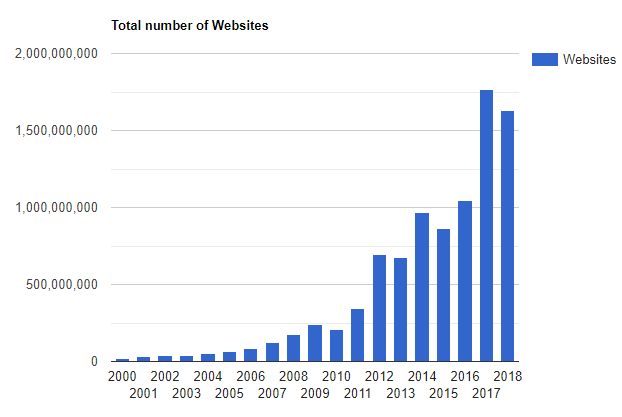
\includegraphics[width=\columnwidth]{images/website-number.png}
            \label{fig:website-number}
        \end{figure}
        
        As of 2020, 43\% of websites were using the popular website builder WordPress, an increase from 13\% in 2011, according to W3Techs \cite{w3}. These services used to make up 1 in 10 websites, but now WordPress alone makes up 4 in 10. The accessibility benefits and simplicity of web builders are likely the reason for their recent surge in popularity. This growth is expected to continue or rise from web 3.0 to 4.0 as the number of websites increases, potentially leading to a situation where technically inexperienced users make up the majority of web developers.
        
        The growing number of developers and non-developers makes understanding UX crucial for maximizing the potential of web applications. UX is a broad psychological concept that is "generally accepted as an extension of the concept of usability" \cite{provost}, with a wide range of applications throughout human-computer interaction (HCI). UX uses user-based metrics, such as the amount of time spent actively engaged with content or the number of events triggered per minute, and perceived opinion based on design to determine whether a UI's design enables effective interaction and meets user requirements. As such, UX is often used in user studies to evaluate the merits and flaws of a given system using either quantitative or qualitative responses. This data can then be used to refactor key web components to improve UX.
        
        The target demographic for web builders is non-developers creating their first website. These non-developers often lack the knowledge and expertise of experienced web developers, and website builders limit their applications to a set of pre-determined tools rather than allowing for the many approaches possible with code. This not only limits the effectiveness and uniqueness of design, but web builder accessibility increases the number of competing sites for small businesses, a popular category among these services \cite{ndukwe}. Increased competition benefits neither small or large businesses, as it decreases their market share of users. Non-unique design only adds to the problem, as websites will look similar to other sites if made with the same web building tools, reducing their brand value, which is closely associated with "customer loyalty and repurchase intention" \cite{mohd-any}.
        
        UX is described by Lynch as a "critical factor in the success of any enterprise" \cite{lynch}. Applications designed with web builders can contribute negatively to UX through poor brand perception, inadequate search engine optimization (SEO), or decreased product value. However, positive UX can help to overcome competition and design challenges. It enhances design principles such as desirability, credibility, and value\cite{morville}. The effective use of these principles can boost site traffic and online purchases \cite{cai} with minimal financial or time investment.

       \begin{figure}[h]
            \caption{Morville's honeycomb \\\hspace{\textwidth} Source: \href{https://commons.wikimedia.org/wiki/File:UX_Honeycomb.png}{Wikipedia commons}}
            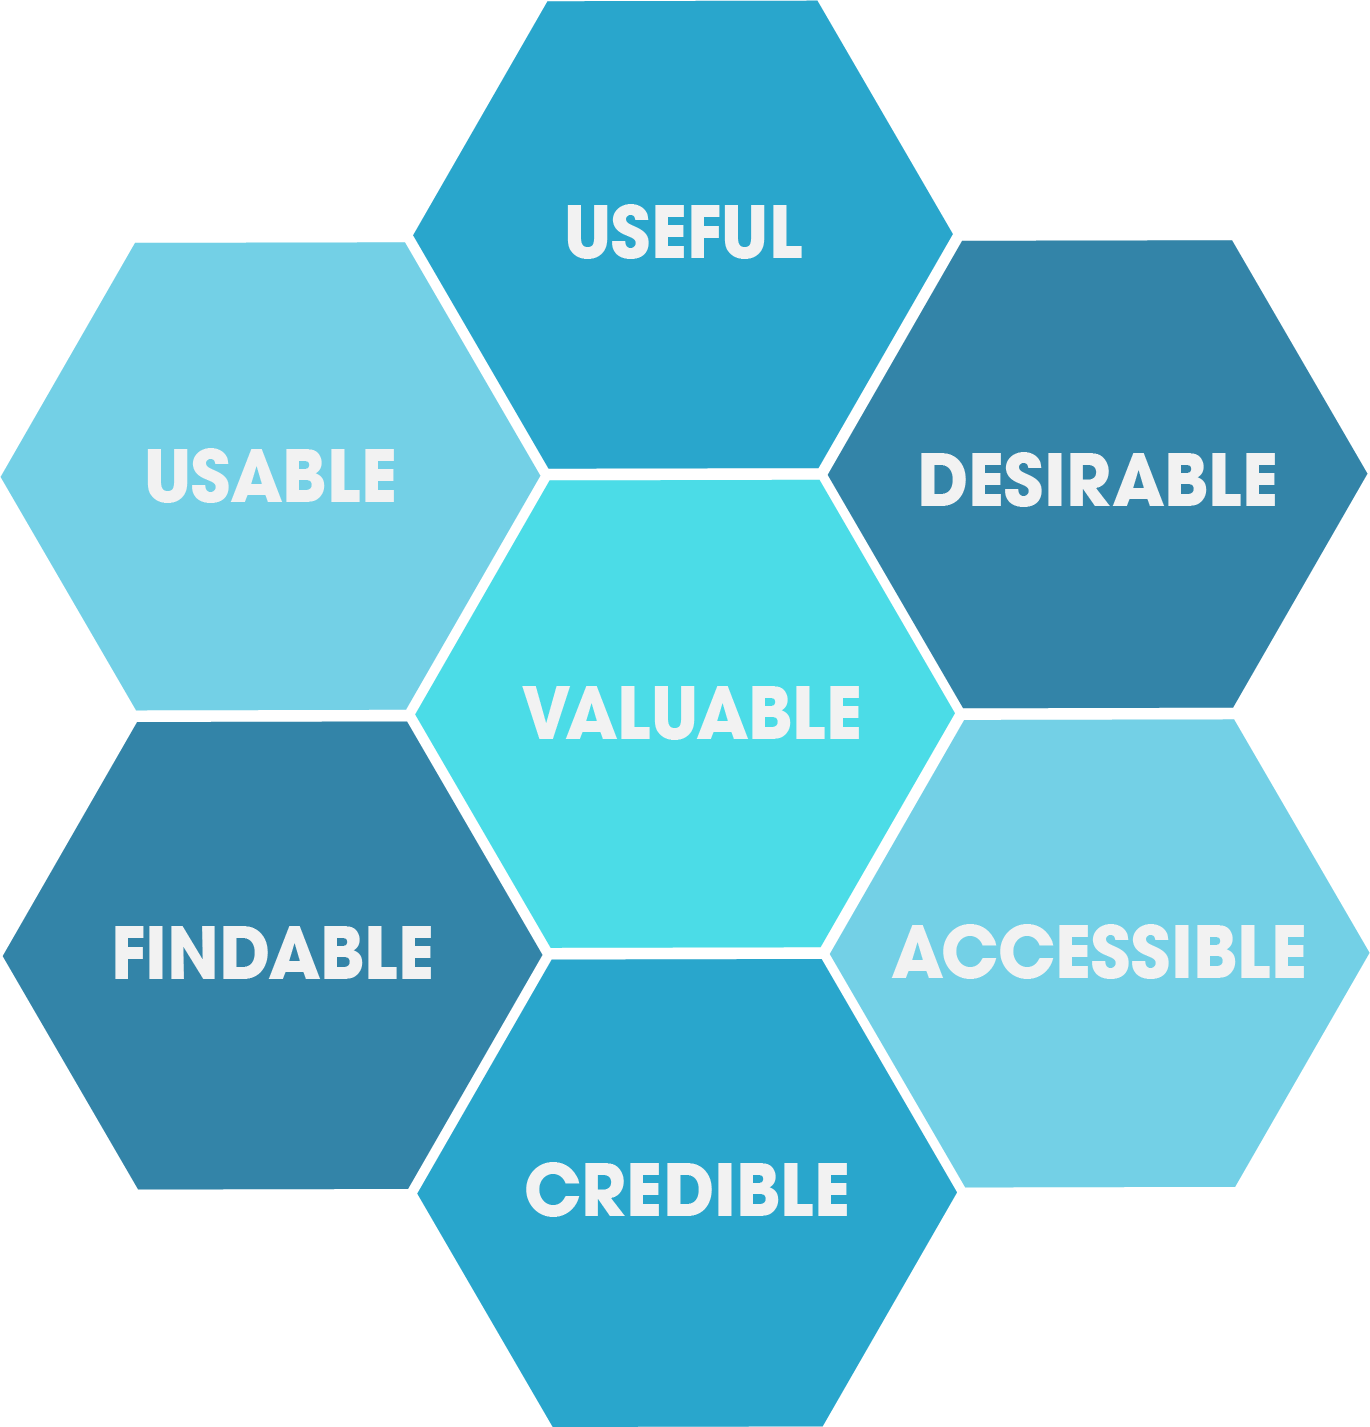
\includegraphics[width=\columnwidth]{images/morvilles-honeycomb.png}
        \end{figure}
                           
        By studying which UI elements and design features improve UX, technically inexperienced users at the core demographic of web builders can benefit from positive UX while still having access to web-building tools. This allows them to maximize the potential success of their website through quality design decisions whilst setting it apart from websites made with the same tools. Therefore, this study aimed to propose a method based on previous research and user study data to identify areas of design that apply to UI and web design to improve UX. The results will be simplified into themes and design elements that the same target demographic can understand, without needing academic knowledge or expertise.

    \section{Literature Review}
        The fields of UI, UX, and web design are crucial in the development of web applications. These areas are broad, encompassing various implementations and methodologies, which result in a range of experiments and results. This literature review examined the current use and necessity of these elements, the practices employed by other researchers to measure them, and how the shortcomings of previous research can be addressed to improve the quality of the study conducted.
        
        It is important to conduct consistent and up-to-date research on these elements, as they are the most tangible ways to assess the strengths and weaknesses of web applications. Furthermore, the web is more accessible and widely used than ever before, for business, education, and social activities. Therefore, it is essential to keep pace with the ever evolving nature of the web to comprehensively understand and improve these elements.
        
        Previous research in these areas has used a range of methods to evaluate the effectiveness of UI and UX design. For instance, Udo et al. \cite{udo} used a qualitative user survey to evaluate the design of e-commerce websites, while Turban et al, \cite{turban} used a literature survey-based approach to assess the major determinants of a successful website. Other researchers have used a combinations of methods, including systematic reviews and expert evaluations, to assess the usability and user satisfaction of web applications \cite{sudiana}.
        
        \subsection{The importance of e-commerce}
            The accessibility of web technologies through website builders has led to numerous new uses, including the selling of online goods or e-commerce as it is referred, which has transformed the way companies interact with customers and compete with one another \cite{slywotzky}. In the past, high-street "brick-and-mortar" businesses dominated the market, but the growing number of web users has made e-commerce "no longer an alternative, it's imperative" \cite{ngamba}. As a result, businesses are creating online counterparts \cite{ullah} in order to stay relevant and make use of new web users.
            
            Using the web as the primary infrastructure offers several positive and negative benefits \cite{kim}, such as lower operating costs online than at a physical location and the increased availability of products outside of high-street operating hours. With web builders increasing competition, businesses need a quick and effective way to create a website and build their online presence. Web builders offer a practical solution, but their discussed benefits and drawbacks may be inadvertently damaging the crucial online presence of businesses.
            
            Designing for maximum UX is critical in e-commerce, as it is heavily relied on for attracting and retaining customers. Researchers Udo et al \cite{udo} and Turban et al have identified navigation, interactivity \cite{udo, turban}, graphic usage \cite{udo}, and loading times \cite{turban} as the most important design factors for e-commerce sites. Navigation and interactivity are particularly important in this context because customers cannot purchase products unless the navigation effectively guides them to the product. Poor interactivity, on the other hand, reduces engagement and leads to lower purchase rates. Using these design factors effectively increases the likelihood of repeat visits and attracts new users \cite{udo}.
            
            Researchers Udo et al. and Merwe et al. have linked good UI \cite{udo} and UX \cite{merwe} to the success of e-commerce, with Cuncliffe stating that "poor web design results in a loss of 50\% of sales and 40\% of recurring users" \cite{cuncliffe}. Given the prominence of e-commerce and the increased competition created by access to web builders, UI and UX become crucial success factors for businesses that rely solely on their online presence. Therefore, enhancing UX through design is a clear way to mitigate the effects of increased competition and should be at the forefront of web design.
            
        \subsection{Design methodologies}
            Since moving away from the fixed-width layouts of web 1.0, new UI principles have aimed to improve accessibility in web applications. Responsive web design (RWD) is one modern principle that has been heavily featured throughout web 2.0 and 3.0, and is described by its creator, Ethan Marcotte, as "creating the optimal viewing experience". RWD enables one codebase to translate designs across any platform, rather than just one \cite{bryant}. Mohamed and Harb \cite{mohamed, harb} discuss how fixed-width designs require a minimum screen size to prevent content from being pushed outside of the page view. RWD uses methods like flexible images, media queries, flexbox and fluid widths to enable developers to make alterations to the design when targeting smaller screen sizes. For example using a fixed width on a desktop but then allowing full width with small margins to minimize whitespace on smaller devices without impacting the contents.
                                    
            RWD became prominent not only because of its modern approach to web design, but also because mobile devices create different user requirements \cite{harb}. Subnic et al estimates that 30\% of users are mobile users, while 25\% are laptop or desktop users \cite{subnic}, later stating that 17\% of sites are responsive. Although, this statistic seems unlikely given the common design principles used in web 3.0, it still limits the number of users across platforms, which is counterproductive to the rising number of mobile users. Based on statistics from Browser Support, Subnic et al lists the most popular resolutions as 25\% 1366x768px and 1900x1200px, while over 30\% are 800x480px \cite{subnic}. This means that mobile devices make up more than laptop and desktop usage combined.
            
            RWD was the first step in creating the trend of "mobile first" design \cite{margea}, the idea of catering design directly to mobile users, popularized in 2010 after Google put forward the idea that their designs should focus on the mobile platform. As previously mentioned, at least 30\% of users are mobile \cite{subnic}, a number that, according to Margea et al and results from StatCounter, surpassed desktop usage in 2016 \cite{margea}. This caused CSS technologies like Boostrap or TailwindCSS to focus on "mobile first" as their targeted styling for developers.
            
            RWD and "mobile first" aim their methodologies at meeting common UX requirements and accessibility. Accessible web applications follow the methods of Accessible Rich Internet Applications (ARIA), a paradigm that Karolic describes as "web for all and web on everything" \cite{karolic}. Because both methodologies focus their practices on accessibility, it makes accessibility a key component in web design. Accessibility may impact UX, site traffic or conversion rates, which are critical factors for businesses given that 42\% of web users make an online purchase within a month \cite{wan}.
                        
            Developers must ensure they understand key design concepts to improve UX. However, web builder users may lack this knowledge. Design trends need to be oriented towards this audience just as they are towards developers. Without design fundamentals, users may unknowingly limit their site's UX. Web builders may make use of design practices like RWD, yet they fail to indicate to their users how these practices have been applied and how they could use them in their future designs.
    
        \subsection{Scoping UX}
            The concept of UX is vast and complex, and there is still no common agreement on its scope \cite{law}, researchers suggest that UX is "still haunted by the challenge of defining scope" \cite{schaik}. Brenyon describes UX as encompassing all the feelings, thoughts, sensations, and actions of engaging in an activity \cite{brenyon}, which makes it difficult to measure metrics. Allam's literature review concluded that UX is challenging and ambiguous due to the impact of perception on bias and its dynamic nature \cite{allam}. Vermeeren also highlights the lack of agreement on the essential characteristics of UX \cite{vermeeren}, while Law, Roto, and Hassenzahl's study found that UX is dynamic, which impacts the methods that can be used to evaluate it \cite{law}.
            
            To limit the scope of UX, researchers use varying techniques. Sudiana et al used many survey papers to identify "43 general factors" that influence UX, with the most common being visual design, information quality, ease of use, and performance \cite{sudiana}. Similarly, Castan˜eda et al. and Cao et al limited their approach to the Technology Acceptance Model \cite{TAS}, using UX to moderate the effect on metrics such as perceived ease of use and perceived usefulness \cite{castan, cao}.
            
            To understand UX design, it is important to move away from vague concepts and limit it's scope, to provide insight to developers and designers so they can improve their design. However, with the growing number of new developers using web builders, users may not understand how these factors apply to their website's design and may not benefit from researchers limiting the scope of UX. Given that ease of use is at the heart of design \cite{sudiana}, new developers should not need technical or academic knowledge to improve their UX.
                        
            Law et al suggests that designing a system of measuring tools with good measurement properties could be a way to address the issue of scope \cite{schaik}. Future research could focus on metrics that target non-developers, rather than defaulting to other academics, and simplify factors to concepts that the audience is likely to understand. For example, where Sudiana et al used information quality, usefulness, and responsiveness as metrics \cite{sudiana}, future researchers could apply these metrics to specific elements of an application that the audience may encounter. For non-technical users, metrics could be presented in a more tangible way, such as "text should be relevant and easy to read," "navigation to any page should be accessible in three clicks," and "your application layout should fit screens smaller than a desktop to promote site traffic." These statements are less vague and more easily understood by less knowledgeable users, increasing the likelihood that they will be able to improve the UX if they understand the factors they can apply to their UI and designs. \\
        
        UI and web design have a range of applications in the modern web, driven by understanding user requirements and using them to improve UX in areas such as accessibility and engagement. Just like developers would improve code, web builders apply previous research findings to their services so that developers can make use of it and improve their UX. However, previous research often overlooks the needs of first-time developers who may have little understanding of design concepts. This means that while they may be able to create their ideal product, they wont be given sufficient understanding of how to further improve their site, as research often offers unfamiliar, broad UX metrics that are incoherent and difficult to comprehend compared to the simple, accessibility-oriented tools they used to create their site.
        
        The key shortcomings of previous UX research is that instead of targeting a specific audience it assumes that the audience already understands design factors that improve UX. This may exclude the growing number of less knowledgeable web builder users, likely to become the majority of web developers. To address this issue, researchers could limit the scope of their experiments using the methods employed by Sudiana et al, Castan˜eda et al, and Cao et al, \cite{sudiana, castan, cao} or they could directly simplify their results to make them more accessible to a non-technical audience. For instance, a non-technical user might benefit more from a statement like "clear, relevant text improved user opinion" than from a statement like "a coherent and applicable typography improves UX." Additionally, this research neglects the varying accessibility needs of users, such as physical or sight-based disabilities, and that these needs can influence the design decisions that benefit their individual UX the most.

        \section{Research Questions}
            \subsection{What are the most effective design elements for improving the UX of web applications?}
                Several design elements can effectively improve the user experience in web applications. The impact of each element on UX varies, depending on the specific requirements of the website. For instance, a forum website may benefit from having more social features, such as upvoting or downvoting, compared to an online wiki. However, there are some overarching elements that are applicable to all types of websites, such as site architecture \cite{ivory}.
    
                Site architecture refers to the overarching design principles that guide the design choices made throughout a website, serving as the site's backbone. Site architecture is a broad concept and can be broken down into factors that contribute to effective UX, such as performance and formatting \cite{ivory}. Performance refers to the computational performance of the website, which is achieved through maintainable coding practices, while formatting focuses on the design of elements such as text, links, and graphics and their distribution across a page \cite{ivory}. These elements are placed in order of importance, known as the visual hierarchy, based on how the site should function. For instance, e-commerce websites often place search bars in the header or hero section of their site to create a "call to action" for searching products quickly.
                
                Each element of site architecture becomes a source of measurement when interacting with users, providing developers with indicators of the effectiveness of their site's design. While any of these elements can impact UX, the design elements that are effective for one site may not be as effective for another. Therefore, it is important to consider the specific needs of the site when deciding on its architecture and visual hierarchy \cite{ivory}. By understanding which elements are most relevant, developers can orient them towards the specific requirements of that site's user. For example, an environmental website may use a largely green colour palette, complementing the website content, while a red colour palette on the same site would have the opposite effect. Similarly, developers can focus on the more important aspects of their site based on their target audience. For example, a clear typography would be much more important on a news website compared to an image gallery website.
    
            \subsection{How can these design elements be understood by a non-technical audience?}
                While understanding which design elements are most effective for a website's target audience is important, this information may not always be helpful to non-technical users. While developers may understand technical terms such as responsive design or search engine optimization, these terms may not provide enough understanding for web builder users. Therefore, design elements must be broken down into tangible design decisions that can be understood by developers of all experience levels.
                
                The implementation of UI and UX design greatly impacts the quality and user engagement of web applications. UI design determines the appearance and overall feel of a web application, while UX design focuses on its usability and functionality. These elements are crucial for determining user engagement and satisfaction with a web application. For instance, Wijaya et al. found that successful websites require a simple, consistent web system that works properly and meets user requirements, based on a System Usability Scale (SUS) \cite{wijaya, SUS}.
                
                Good UI design can enhance the aesthetics of a web application through its content, functions, and usability \cite{gunawan}. This can make it more visually appealing and improve the overall UX, resulting in increased user engagement and satisfaction, as users are more likely to use and enjoy a well-designed and aesthetically pleasing web application. Effective UX design focuses on making a web application easy to use and navigate \cite{gunawan}, which can lead to improved user satisfaction and engagement, as users can quickly and easily accomplish their desired tasks within the application. Therefore, UX and UI determine the quality of web applications through metrics such as user engagement, which is influenced by the implementation of design.

        \section{Hypotheses}
            There are two key hypothesis for this experiment. The first is that "There will be a significant different between the proportion of positive and negative results between artefacts A and B" [\autoref{tab:hypotheses}]. This is likely due to the informed design of artefacts A and the role of individual perception in UX related studies, which in combination will cause variations user-based metrics. The outcome of the first hypothesis will determine the second: "Artefact's A design is more effective than artefact B" [\autoref{tab:hypotheses}], as a higher proportion of results will determine key areas that either artefact is more successful in. However a statistical test will give the overall measurement of proportions and thus reject the second null hypothesis.

            \begin{table}[ht]
                \caption{Hypotheses}
                \centering
                \renewcommand{\arraystretch}{1.5}
                
                \begin{tabular}{p{0.32\linewidth} | p{0.32\linewidth} | p{0.21\linewidth}|c|c|c|}
                    \hline
                    \textbf{Hypothesis} & \textbf{Null Hypothesis} & \textbf{Data source} \\ \hline
                    There is a significant different between the proportion of positive and negative results between artefacts A and B & 
                    There is no significant different between the proportion of positive and negative results between artefacts A and B & 
                    Statistical test, column graph comparison \\ \hline
                    
                    Artefact A's design is more effective than artefact B & 
                    Artefact A's design effectiveness is less than or equal to artefact B & 
                    Statistical test, proportion of results from user based metrics \\ \hline
                \end{tabular}
                \label{tab:hypotheses}
            \end{table}

    \section{Artefact}
        The artefacts used in paper's study were online e-commerce websites, artefact A made with specific design alterations [\autoref{fig:index-wireframe}] informed by the literature review, while artefact B is a similar site made using a website builder. Artefact B is included for comparison only and is not credited as the work of this paper; only artefact A will be discussed. Because e-commerce is highly relevant to the web industry, it was deemed as the most appropriate website genre to accurately understand it's design merits based on user opinions. This experiment provides valuable insights for not only this paper, but also for users applying the results to their own work. The main features of this application are standard elements commonly seen in e-commerce sites, such as login, registering, searching, filtering, a cart and checkout system, along with design alterations including; images in and out of the scene, a colour theory-based colour palette, animations, a call to action section and an altered page structure to be used as variables in the experiment. Both the applications source code and database are cloud-hosted using Heroku and ClearDB.

        The technologies used to create artefact A are ReactJS and TailwindCSS for the front-end because of React's increased performance and re-usable approach to HTML and client-side JavaScript, while TailwindCSS reduces development time by using a shorthand CSS syntax. The back-end uses Node.js, ExpressJS, and MySQL because Node offers a vast array of packages and tool for development while Express offers additional routing and server functionality. While the user, product and checkout data is stored in a linear, logical format that is better suited to SQL than NoSQL. All authentication systems like login, registering and checkout forms are encrypted before being stored using Node.js's Crypto package, utilising hash, pepper and salting inputs via an environment file. All HTTP requests to database endpoints are handled using Axios given it's improved functionality over standard HTTP fetch requests.

        \begin{figure}
            \caption{Index page wireframe \\\hspace{\textwidth} Reference:\href{https://github.falmouth.ac.uk/JH248828/Comp320_A1-Comp360_A1/tree/documentation}{JH248828/Comp320\_A1/documentation} \\\hspace{\textwidth}}
            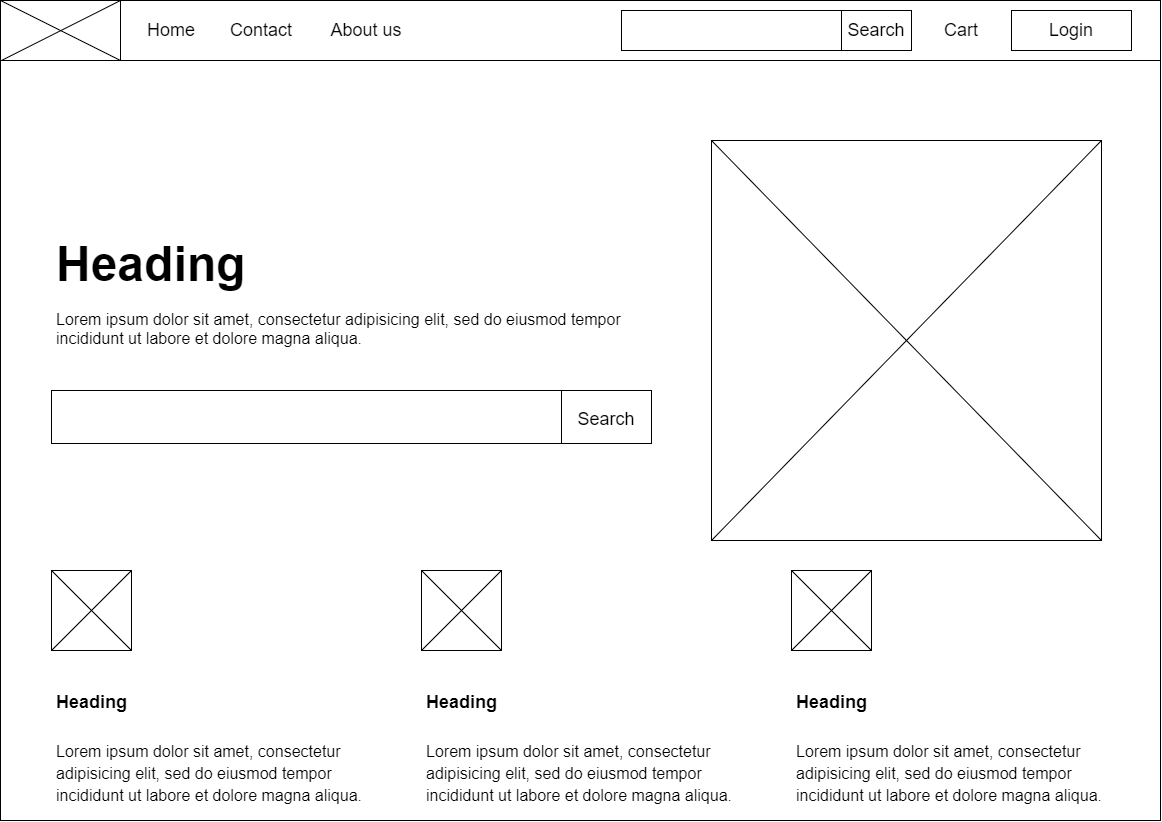
\includegraphics[width=\columnwidth]{images/artefact/index-wireframe.png}
            \label{fig:index-wireframe}
        \end{figure}

        \begin{figure}[]
            \caption{Use case diagram \\\hspace{\textwidth} Reference: \href{https://github.falmouth.ac.uk/JH248828/Comp320_A1-Comp360_A1/tree/documentation}{JH248828/Comp320\_A1/documentation}}
            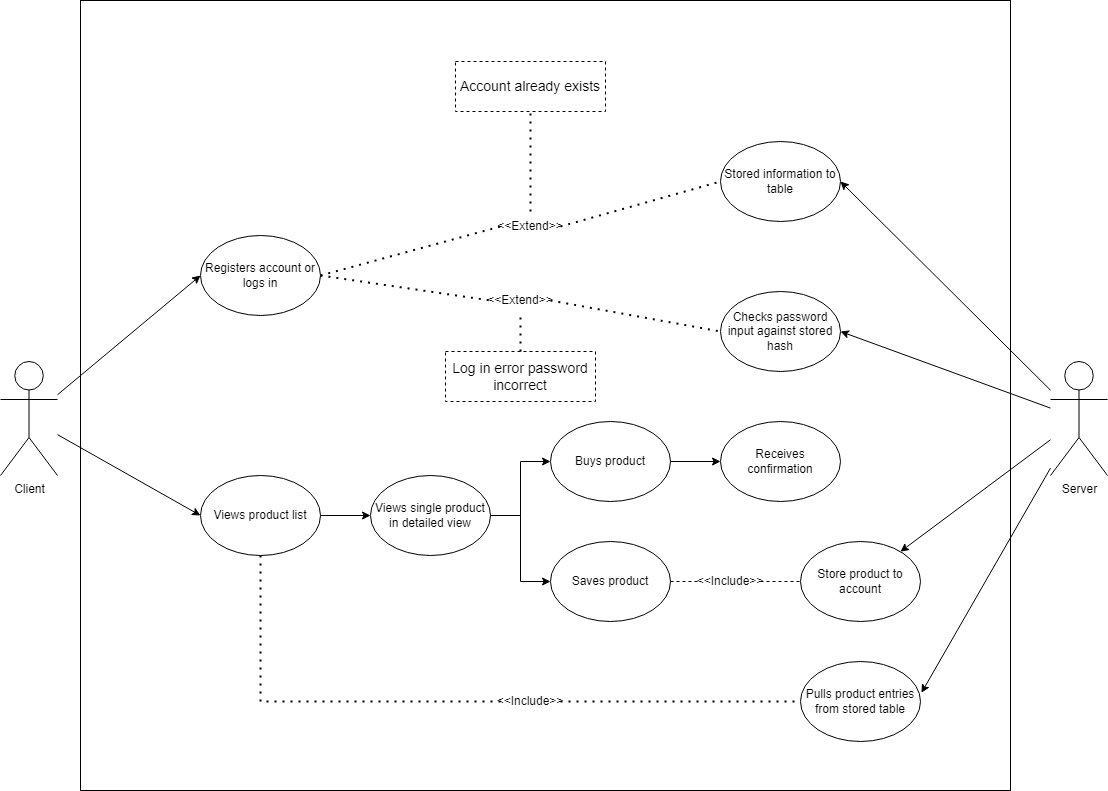
\includegraphics[width=\columnwidth]{images/artefact/use-case-diagram.png}
        \end{figure}

        \subsection{Validation and verification}
            The development lifecycle used for artefact A was an incremental approach, which allows the artefact to be divided into sections based on each feature, these could then be improved upon iteratively, rather than completed everything at once like in waterfall. This development cycle was chosen over the similar agile approach because, although it follows many of the same practices, it is better suited to a situation where the requirements of the artefact are unlikely to change as a result of design constraints. The incremental approach also allows for individual features to receive feedback throughout the development process, which can then be refactored and altered based heuristic evaluations or other forms of feedback such as the one conducted before the study in \autoref{fig:preliminary-heuristic-analysis}.
    
            The testing areas for this artefact included unit testing, integration testing, acceptance testing, and usability testing, the most significant of being acceptance and usability:
            \begin{enumerate}
                \item Unit testing was used to manually test individual features by interacting with them, including the cart, search, checkout, and product systems. Automated systems can also be used to help with this process.
                \item Integration testing also manually tested the functionality of site-wide features, such as testing the search system with product pages or the cart displaying on the checkout page.
                \item Acceptance testing could be performed manually but was measured through heuristic evaluation to verify that the site meets user requirements and expectations.
                \item Usability testing used the same methods as acceptance testing but was measured through developer tools and verified accessibility and responsive web design practices.
            \end{enumerate}
    
            \begin{figure}[h]
                \caption{Preliminary heuristic analysis conducted 26/11/22 \\\hspace{\textwidth} Reference: \href{https://github.falmouth.ac.uk/JH248828/Comp320_A1-Comp360_A1/tree/documentation/hueristics}{JH248828/Comp320\_A1/documentation}}
                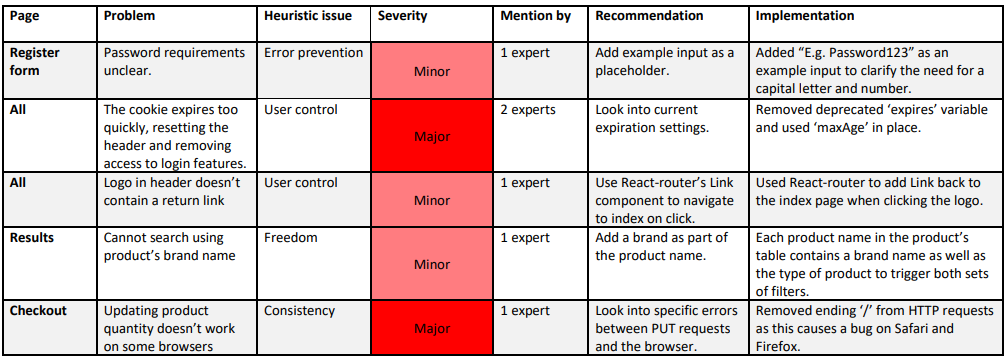
\includegraphics[width=\columnwidth]{images/testing/heuristic-analysis.png}
                \label{fig:preliminary-heuristic-analysis}
            \end{figure}
    
    \section{Methodology}
        The basis for this paper's study on design decisions that improve UX and the current shortcomings of web builders is the literature review. The review provided insight into which metrics should be used in the study and informed the design decisions artefact A. The study is divided into two parts: an A/B test between two similar artefacts and a thematic analysis of the qualitative results to identify trends between them.
        
        The A/B test uses this paper's artefact (artefact A), an electronics e-commerce site, and a competing site of the same genre made with a website builder (artefact B), between two study groups. As discussed A test has various alterations to its design, targeting the e-commerce design factors listed by Udo et al \cite{udo} and Turban et al \cite{turban}, to determine their impact on UX. Both study groups were tasked with selecting several products from different categories, either by brand name or product type, and adding the products to the site's basket or cart.
        
        Participants were tasked with reaching the final stage of each site's life cycle, either a confirmation page or the checkout form page. Purchasing products was not required and was actively discouraged, but users could have filled out the checkout form without providing their data to test it's functionality. Retrieving several different products allows most, if not all, site features to be used, such as searching, filtering, updating, and deleting products, giving users freedom of approach. During the test, participant's clicks were measured using a "click map," a digital heatmap showing where clicks were most common. This provided insight into which products or systems were most active and allows conclusions to be drawn specific to those elements. Due to rights permissions, this was only applied to the A test, but it still determines the effectiveness of the design decisions specific to artefact A.
        
        After completing the task, participants filled out a qualitative answer sheet based on the most common UX metrics from the 43 papers that Sudiana et al \cite{sudiana} surveyed when creating their metrics [\autoref{tab:metrics-table}]. After the answers were collected from each study group, a thematic analysis was performed to identify correlations and patterns between the metrics and the artefacts. This data, along with the click maps, was used to determine which elements in each artefact were the most influential during the tasks and was insightful into how the artefact's design impacted its UX. The results were categorised and linked to page sections (e.g., hero, authentication forms, search system) to measure their effectiveness in the study group's task.

        \begin{table}[ht]
            \caption{qualitative metrics used in experiment}
            \centering
            \renewcommand{\arraystretch}{1.5}
            
            \begin{tabular}{p{0.32\linewidth} | p{0.21\linewidth} | p{0.32\linewidth} |c|c|c|}
                 \hline
                 \textbf{Question} & \textbf{Targeted metric} & \textbf{Expect results} \\
                 \hline
                 What was your opinion on the colour scheme? & Colour scheme & Colour compatibility with content \\
                 \hline
                 What was your opinion on the quality of the information? & Typography and relevant information & Text relevance, quantity of text \\ 
                 \hline
                 How easy was the site to use? & Accessibility & 3-click rule and ARIA compliance \\
                 \hline
                 How was the sites performance? & Computational performance & Site's load time both initially and between pages \\
                 \hline
                 What was your opinion on the site's layout? & Structure and aesthetics & Clarity of structure, merits and flaws of the overall design \\
                 \hline
                 Did the site's design fit your device? & Responsive web design & Maintainability of the sites structure, responsiveness between devices \\
                 \hline
                 Were the error systems suitable and informative, if encountered? & Error systems & Insightfulness of error messages, missing error systems \\
                 \hline
                 How consistent was the site's design? & Consistency & Consistency of styling and design across all pages \\
                 \hline
                 Did the sites features work the way you expected? & Functionality & Search system and checkout effectiveness \\
                 \hline
            \end{tabular}
            \label{tab:metrics-table}
        \end{table}

        The study's research philosophy was interpretivism, as UX was the primary focus underlying this research, and its ontology is based on individual perceptions, as is the case with most studies involving participants. It's epistemology, which relies on valid knowledge through consensus of opinion, is suitable for qualitative studies as it allows participants to project a wide range of ideas. The method of induction is used to form conclusions as it can assume outcomes based on common themes from systematic reviews, commonly used in UX research. By falsifying the metrics of each artefact, it can be concluded whether the alterations impacted UX or not.
        
        Given the interpretivism-style approach used in the study, the potential spectrum of answers between two study groups and qualitative results is broad. A thematic analysis can help condense the results into themes that identify contributing design choices instead of broad opinions. A/B testing is a simple and effective method of comparison between the methods of this paper and the methods used in industry web builders. Participants can easily understand the strengths and weaknesses of each design and provide detailed answers that can improve the results compared to a quantitative approach. The experiment wasn't extended beyond an A/B test or thematic analysis as scope is already a prominent issue in measuring UX. The aim of using simpler methods to condense the scope is to appeal to the growing number of non-technical users who can apply the results without requiring substantial technical knowledge.

        A potential limitation of the study is that the findings may not be applicable outside of the e-commerce genre they were recorded for. This means that design elements that benefit e-commerce websites may not be relevant to other types of websites. To address this limitation, the user study included a broader, more diverse range of participants across several disciplines or could have used additional data collection methods, such as regression analysis, to measure the effectiveness of design elements across different genres. This could help to improve the generalizability of the study's findings across any genre.
        
        \subsection{Ethical considerations}
            Both the A and B tests required active participants to provide feedback. To conform to the General Data Protection Regulation (GDPR) \cite{gdpr}, a disclaimer was included at the beginning of each form informing participants that their responses will be part of this study. The participant's personal information was anonymized, and instead of giving their name, participants were named participants 1, 2, 3, and so on, with two of each participant across each study group. For example, group A had a participant A.1 and group B had a participant B.1. Participants could still provide a name, but this was strictly for referencing purposes only, and didn't have to be their real name. Participants were given a brief detailing an overview of the study and its objectives. Following this a consent form had to been signed and dated prior to participating in the study, detailing the risks and an overview of their task. Participants were given a 3 week grace period, upon completion where they have their data deleted. After this period they were kept as part of the study, although they could request a copy of their data at any time. After the study participants were given a debrief thanking them and indicating the key findings their participation would help achieve. Before the study begin ethical approval was secured from both the researcher's supervisor and module lead assessing the details of the; participant requirements, risk assessment, demographic detailing, brief, debrief and consent form provided by the study's conductor.
            
            The artefacts contained login and registering systems, which could store personal information, but participants were instructed complete their tasks without using them, as they were not required for the task. To ensure compliance, they were logged into a pre-made admin accounts for artefact A, and the database was cleared after the study. For artefact B, the task could be completed without the login system so this wasnt an issue. If however they did create an account their data was removed from the study.

            The study's data was collected through online forms via a secure link. None of the participant's personal information was stored on this form. Only the qualitative answers to each question in table \ref{tab:metrics-table} and a placeholder for referencing should they have choosen to withdraw. These results were exported to a CSV file and stored on Falmouth University's OneDrive. The click map data didn't require any user information as it only recorded click locations and interactions from users on the site. To ensure that this data was only from participants, the click map was activated when the study began and stopped after.

        \subsection{Data management}
            To test the significance of each null hypothesis, a two-sample proportional test was conducted. This test compared the proportion of positive results to the proportion of negative results using R's 'prop.test' function. If any column gave a higher number of positive results than negative results, it supported the first hypothesis [\autoref{tab:hypotheses}]. Positive and negative results were plotted as a column chart using R's 'ggplot' library, with one metric per column. To test the reliability of the data against chance, a Benjimini-Hochberg adjustment was applied.

            The dependent variable was the number of positive or negative results, and the independent variables were the design metrics listed in \autoref{tab:metrics-table}. Each artefact had its own graph comparing the number of positive and negative results for each metric [\autoref{tab:metrics-table}]. The first bar represented the number of positive results, while the second bar represented the number of negative results. The x-axis was the metrics [\autoref{tab:metrics-table}] and the y-axis was the number of participants. The artefact with more positive results under the same metric suggested that its design benefited that metric better and help support either hypothesis [\autoref{tab:hypotheses}]. The results of the qualitative answers provided by the questionnaire, were analyzed using thematic analysis. This analysis indicated which design elements contributed to the outcome of the results and, by extension, why one artefact might perform better than the other under the same metric.

            The A/B test's sample size used a large effect size of 0.8, resulting in 26 participants for each study group, totalling 52 participants. The larger effect size was due to qualitative answers providing more detailed data then quantitative data, as well as the ability for users to approach the experimental task in different ways, resulting in longer and more varied responses. Additionally, using the same questions for both artefacts provides enough varied responses to allow for patterns to be drawn and assumptions to be made in the thematic analysis, enabling conclusions to be drawn about either an individual artefact or both. A larger sample size may have impacted the experiments running time, as qualitative data generally requires more time investment from participants compared to quantitative data. On the other hand, a sample size that is too small may effect the p-score given by the Benjimini-Hochberg adjustment, suggesting more results from chance. The sample maintained standard error probabilities of 0.05 as they were unlikely to be affected by the requirements or task in the experiment.
            
            \clearpage
            
            \begin{figure}
                \caption{G power sample size}
                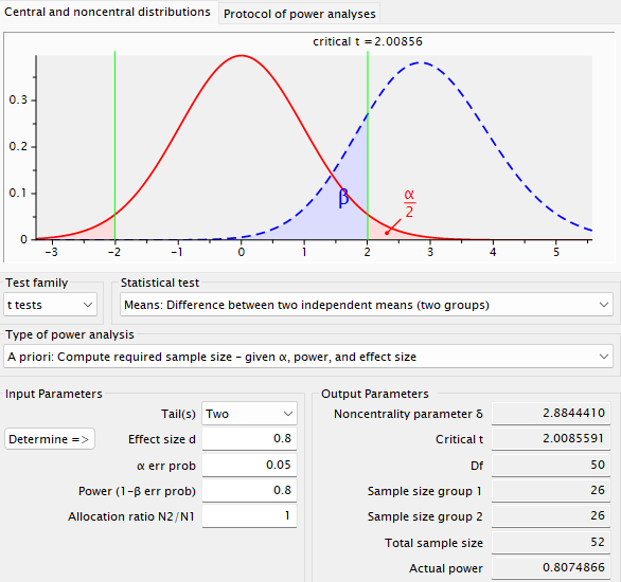
\includegraphics[width=\columnwidth]{images/data/sample-size.png}
            \end{figure}
            
    \section{Results}
        The approach used to collect and analyze data followed the outline set in the methodology previously. To make Artefact B a similar site to Artefact A, a Shopify test theme was used. Shopify is a website builder specifically for e-commerce sites, and it has several themes available to test that are functionally the same as live sites. To make the test results differ, the artefacts themselves had several key differences:
        
        \begin{enumerate}
            \item Artefact A used a light purple and blue colour palette, whereas Artefact B used a mostly dark black and white colour palette.
            \item Artefact A used a search bar and image for its landing page, while Artefact B used an image carousel.
            \item Artefact A used rounded images and elements, whereas Artefact B used sharper block elements.
            \item Artefact B sold a limited range of products and so showed all its product information on the index page, whereas Artefact A had a dedicated page for each product.
        \end{enumerate}

        \begin{figure}[h]
            \caption{Artefact A \\\hspace{\textwidth} Reference: \href{http://www.tech-terminus.me/}{Tech Terminus}}
            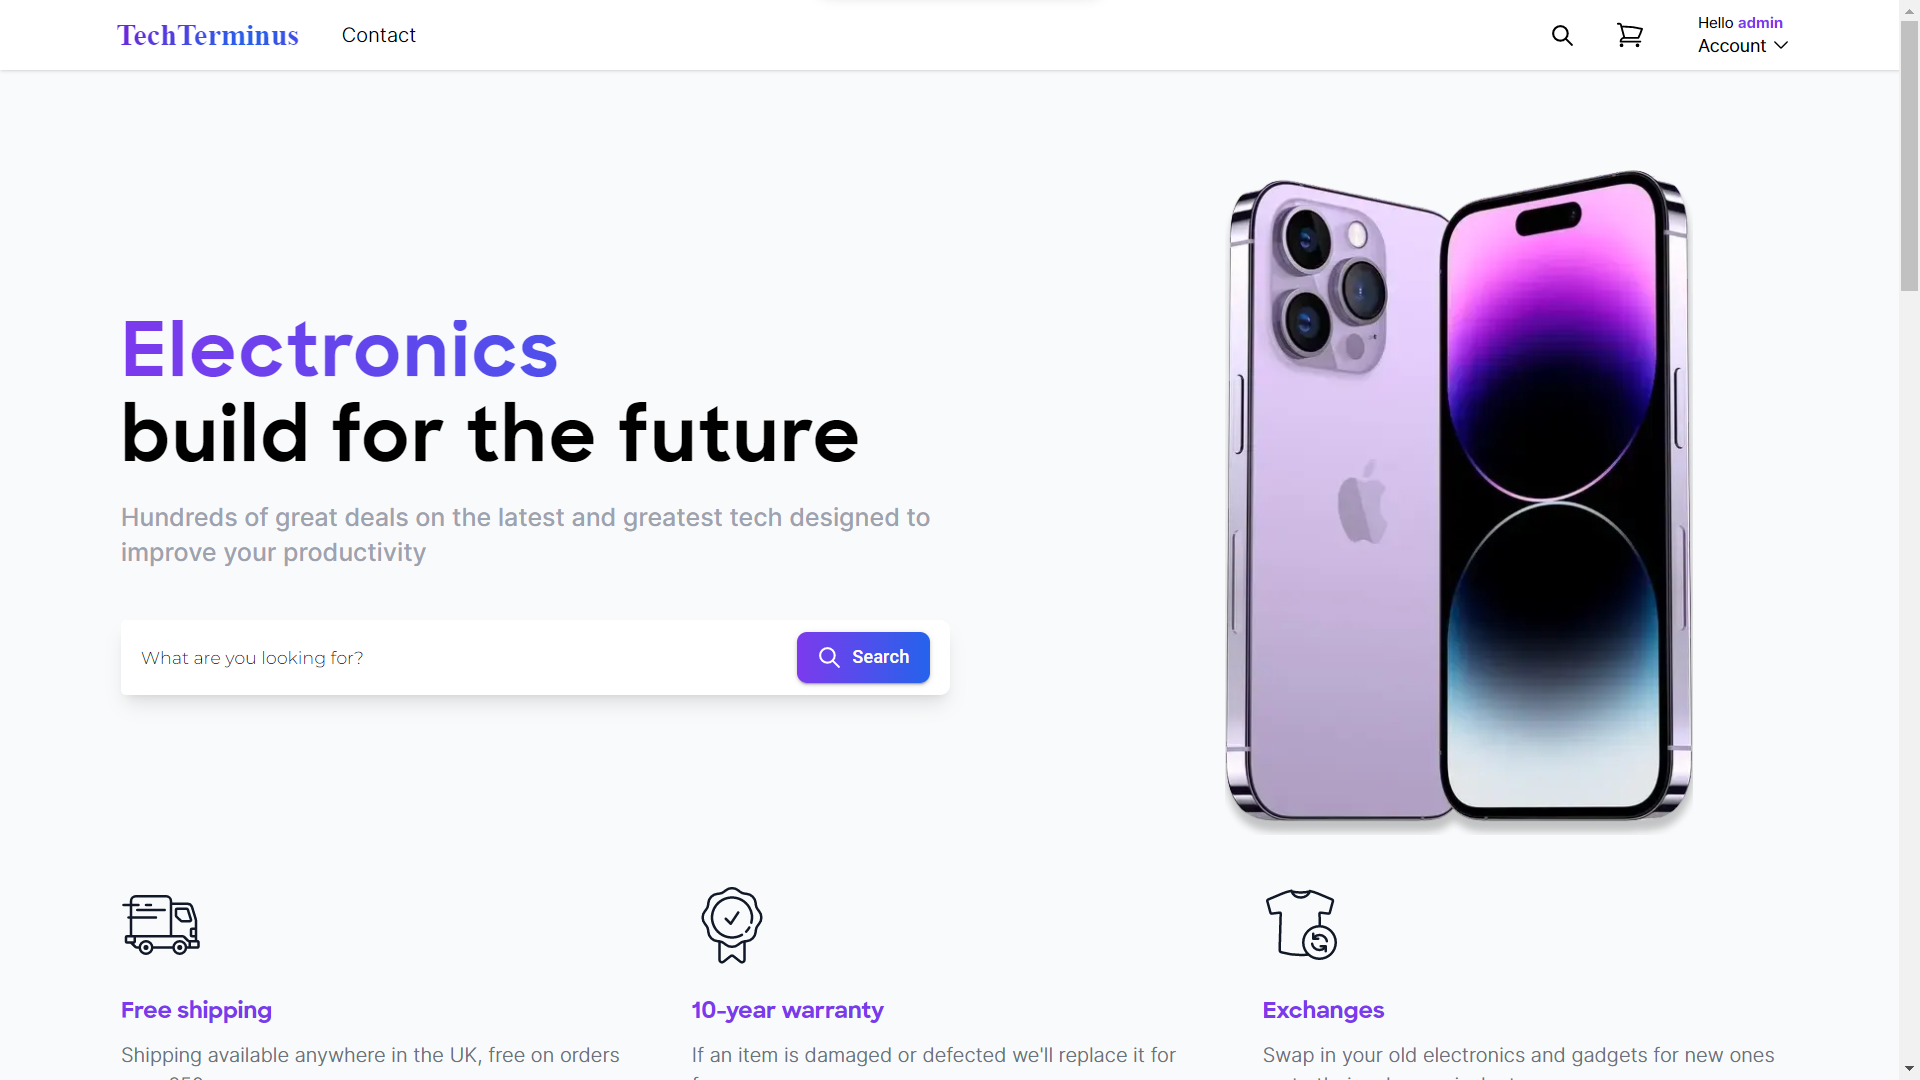
\includegraphics[width=\columnwidth]{images/artefact/artefact-a.png}
        \end{figure}

        \begin{figure}[h]
            \caption{Artefact B \\\hspace{\textwidth} Reference: \href{https://beyours-theme-tech.myshopify.com/}{Shopify theme}}
            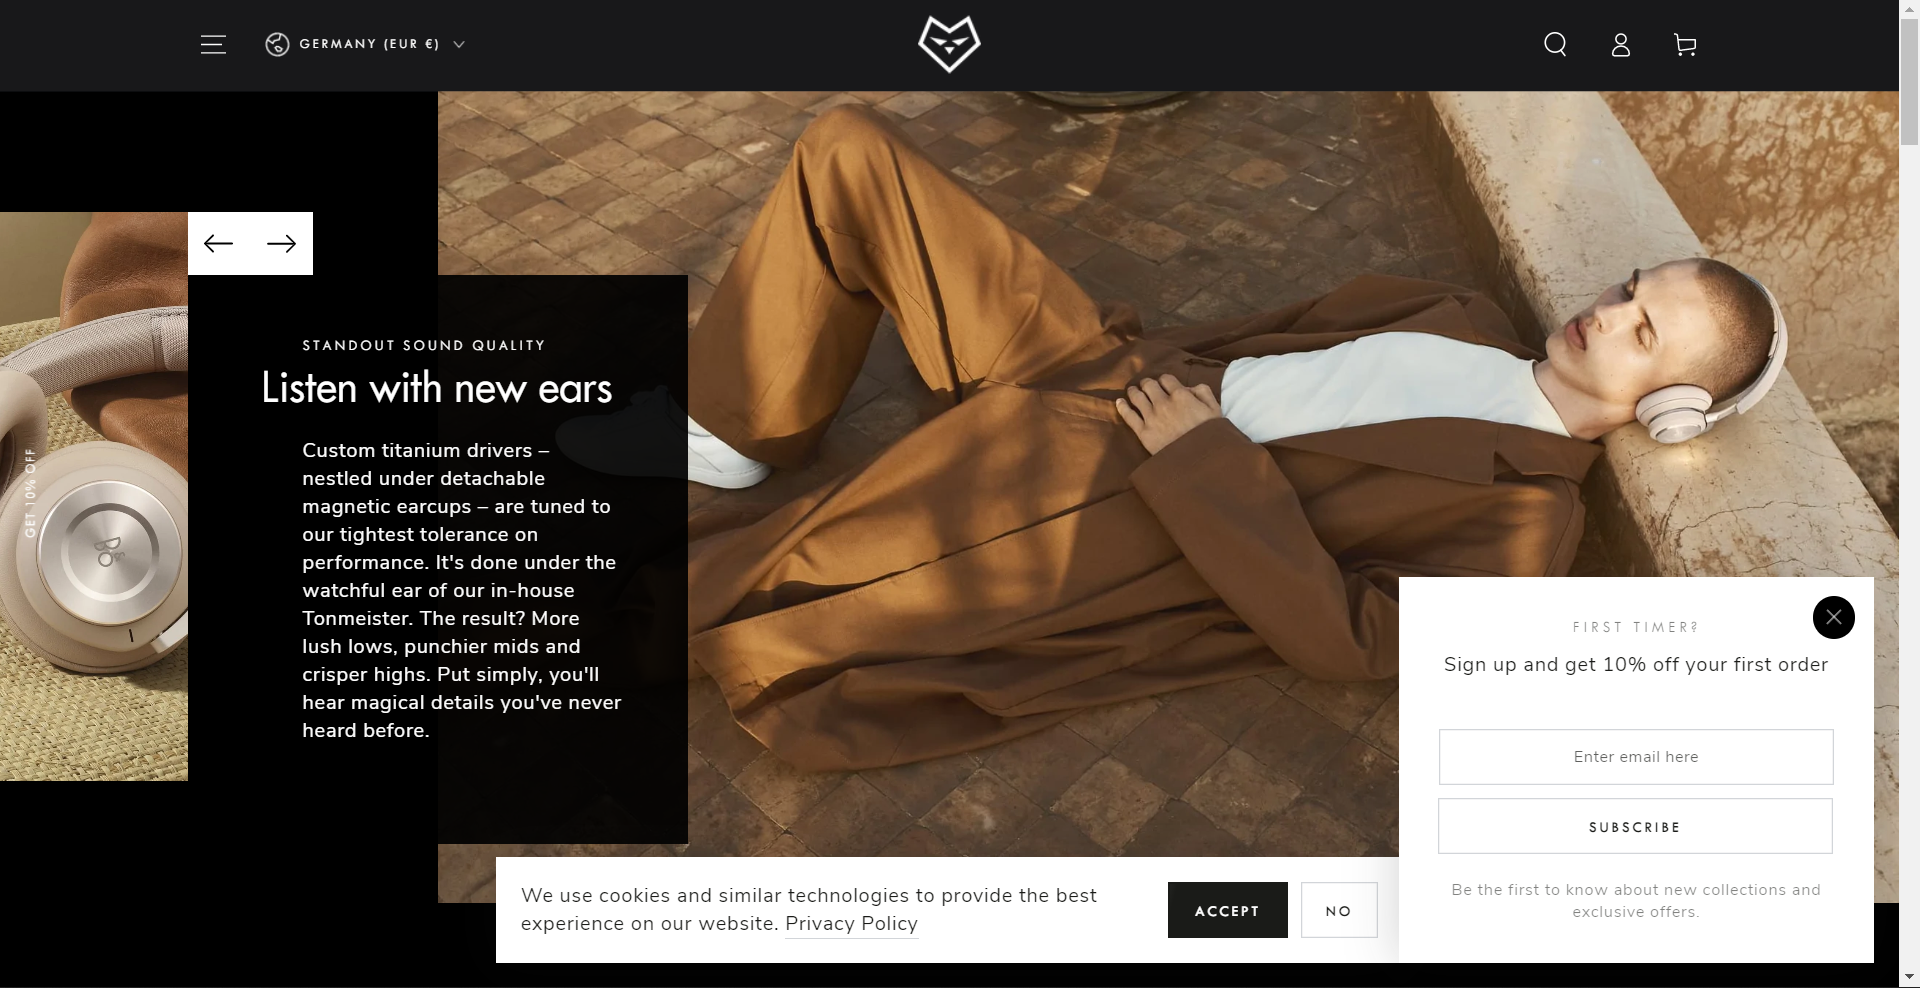
\includegraphics[width=\columnwidth]{images/artefact/artefact-b.png}
        \end{figure}

        The study itself followed the same approach mentioned in the methodology section, an A/B test with 26 participants per study group. Participants were assigned a A or B's website to complete a task on and then had to answer a set of metrics based on the website's design and functionality. The demographic of participants were largely undergraduate university students, specifically those under the computing or games development disciplines, meaning they had a higher than average level of technical knowledge. This was key in the test, as participants would need to understand the role of common e-commerce website features like searching or adding products to a cart in order not to impact the test results based on individual ability rather than the functionality of either artefact. The study was as inclusive as possible, not requiring specifics such as age, gender, or ethnicity.
        
        The data was collected via a Microsoft Forms questionnaire given to each of the two study groups containing the metrics outlined in the methodology section [\autoref{tab:metrics-table}]. This was then processed through Microsoft Excel, where each answer from each participant was given a mark based on the positivity of their response. "P" was given for a mostly positive response, and "N" for a mostly negative response. Given that this method may create an element of bias, the marks were only given as column values for each column in the following column charts [\autoref{fig:group-a-plots}, \autoref{fig:group-b-plots}]. The full responses, regardless of these marks, can still be analyzed in appendix: \autoref{tab:study-data}. After processing responses, they were exported as a CSV file into R studio, where it could form one the two column charts. Both charts used the positive and negative responses from each study group, one for group A and one for group B, respectively. The data had each positive and negative results counted and added to a data frame then used the "ggplot" function to create a column graph. The data also used a two-sample proportional test to determine differences between the proportion of positive results against the proportion of negative results for each graph and a Benjimini-Hochberg adjustment to account for the rate of false discovery.

        \clearpage
        
        Out of the 52 participant sample size, 42 participants conducted the study. Group A received 21 total participants [\autoref{fig:group-a-plots}], and Group B also received 21 participants [\autoref{fig:group-b-plots}].

        \begin{figure}[h]
            \caption{Group A plots}
            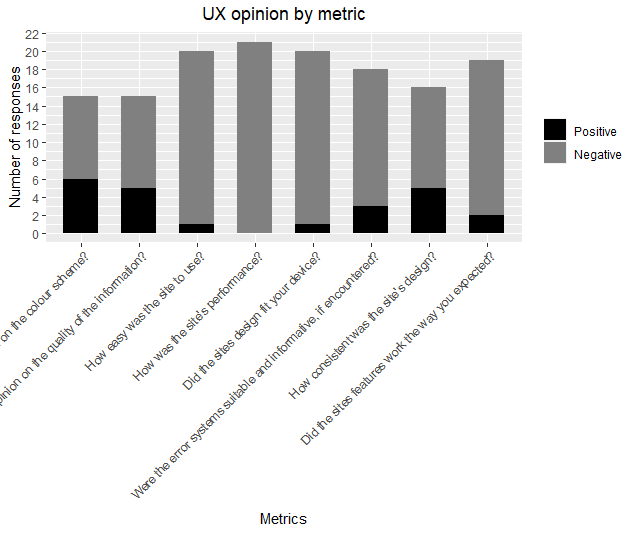
\includegraphics[width=\columnwidth]{images/data/group-a-plot.png}
            \label{fig:group-a-plots}
        \end{figure}

        \vspace{-10mm}
        
        \begin{figure}[h]
            \caption{Group B plots}
            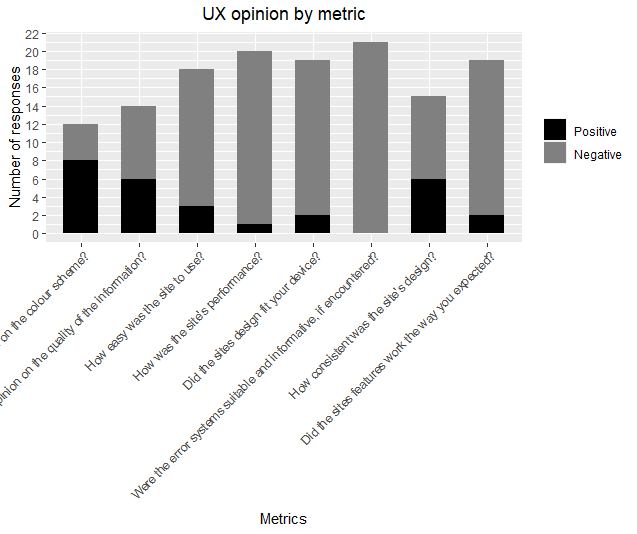
\includegraphics[width=\columnwidth]{images/data/group-b-plot.png}
            \label{fig:group-b-plots}
        \end{figure}

        \vspace{-7mm}

        \subsection{Limitations}
            The results of the study have been impacted by several limiting factors. The results themselves contain varying responses. While this is the nature of qualitative data, factors like the individuals' enthusiasm for the study and their relationship to the conductor are likely to affect the quality of each answer given. Not reaching the sample size also affects the quality of the study. More data collates more findings and increases room for discussion. Had this been a funded study with several conductors or had a larger scope, this sample size would have been more attainable. The conductor's individual ability also impacts the quality of Artefact A, leading to the potential for more negative responses relating to the individual's technical ability rather than the artefact's design pitfalls.

    \section{Findings}
        Before analyzing the findings of the two figures [\autoref{fig:group-a-plots}, \autoref{fig:group-b-plots}], the limited sample size should be acknowledged. Given that both groups were missing an additional 5 participants each it gives each individual's answer a slightly greater effect size. Whilst this is negligible this should be accounted for when concluding from this data.
        
        Each of the metrics used in the study saw varying percentages of negative and positive responses. Metrics such as "accessibility", "computational performance", "structure", "error systems", and "RWD" showed little fluctuation when compared to other metrics like "colour scheme" [\autoref{tab:metrics-table}]. These variations indicate that the metrics had different levels of influence on UX based on their role in the artefact. For example, "performance" and "error handling" are mostly handled on the server-side of a web application and, as a result, have far fewer interactions with the client-side than a metric like "structure and aesthetics". After thematically analyzing the results, metrics that didn't have an immediately apparent or clear roles within the application resulted in themes of ineffective responses such as "no performance issues" or "I didn't encounter any errors," which by default create positive UX, but provide little feedback for the developer.

        Survey papers conducted by Udo et al and Sudiana et al found similar results. Udo et al found "visual design, information quality, and ease of use" \cite{udo} to be the most common metrics in other surveyed UX related studies, while Sudiana et al, using the same methodology, found "layout, typography, colour, and aesthetics" to be the most common factors \cite{sudiana}. These are all client-based metrics and support the finding that server-side metrics have limited variation compared to client-side metrics.

        The remaining client-side metrics include: "colour scheme", "typography", "consistency" and "functionality" [\autoref{tab:metrics-table}]. All of these metrics saw large variations between the two artefacts. Artefact A performed better in all criteria aside from "functionality" where the results were even. These variations are likely a results of the comparison of approaches between artefact A's informed design alterations and the approach of artefact B's design as well as individual preferences such as preferring light colour pallets against dark colours pallets.

        \begin{table}[ht]
            \caption{Statistical test results and adjusted p-values for Group A and Group B}
            \centering
            \begin{tabular}{|c|c|c|}
                \hline
                \textbf{Group} & \textbf{Proportional test p-value} & \textbf{Adjustment p-value} \\ \hline
                A & 0.04566735 & 0.04566735 \\ \hline
                B & 0.004929431 & 0.004929431 \\ \hline
            \end{tabular}
            \label{tab:statistical-results}
        \end{table}

        In addition, the data gathered from the statistical test indicates that artefact B performed worse overall rejecting the second null hypothesis [\autoref{tab:hypotheses}], as it contained more negative scores across the metrics [\autoref{tab:metrics-table}] than artefact A [\autoref{tab:statistical-results}]. Group A's p-value was 0.04566735 at an error rate of 0.05, suggesting slight difference between the proportions of positive and negative results. However, group B's p-value was 0.004929431 at the same error rate, making the proportions highly significant. This indicates that UX on this website varied drastically compared to artefact A supporting the hypothesis that "There was a significant different between the proportions of results between each artefact" [\autoref{tab:hypotheses}]. While, this may be a result of the individual's preferences, it still supports the first hypothesis and as a result further supports the second hypothesis in determining that one artefact was more effective based on its design than the other [\autoref{tab:hypotheses}], because artefact A's results were less significant that artefact B.
        
        The heatmap data gathered for artefact A using Microsoft Clarity provides insights into the most used UI elements in that artefact. Areas with red or yellow rings indicate the most active points, whereas blue or purple rings indicate less active locations. The heatmap suggests that the incentives were the most clicked UI element, followed by the search and login features [\autoref{fig:heatmap}]. All of these features were within the first page load, and research into eye-tracking and typical website layouts suggests a reason for this. Based on eye-tracking data, users tend to look from left to right, starting in the top left corner, moving to the middle of the page, and finally to the top right \cite{djamasbi}. This is before any notable interactions are made by the user. Therefore, any features within the first page are likely to be interacted with, as shown by the features outside of the first page, such as the products, that received fewer clicks [\autoref{fig:heatmap}].

        It is equally important that pages match the typical website structure, universal to most websites, to take advantage of eye-tracking, such as the logo being in the top left, account information on the right, and the header and footers respectively at the top and bottom of the page, with a large hero section containing a call to action \cite{nevarez}, in this case, a search bar. These two factors in combination indicate that the first page a user sees is by far the most important in website design and the majority of design should focus this section.

        \begin{figure}[H]
            \centering
            \caption{Artefact A heat map data}
            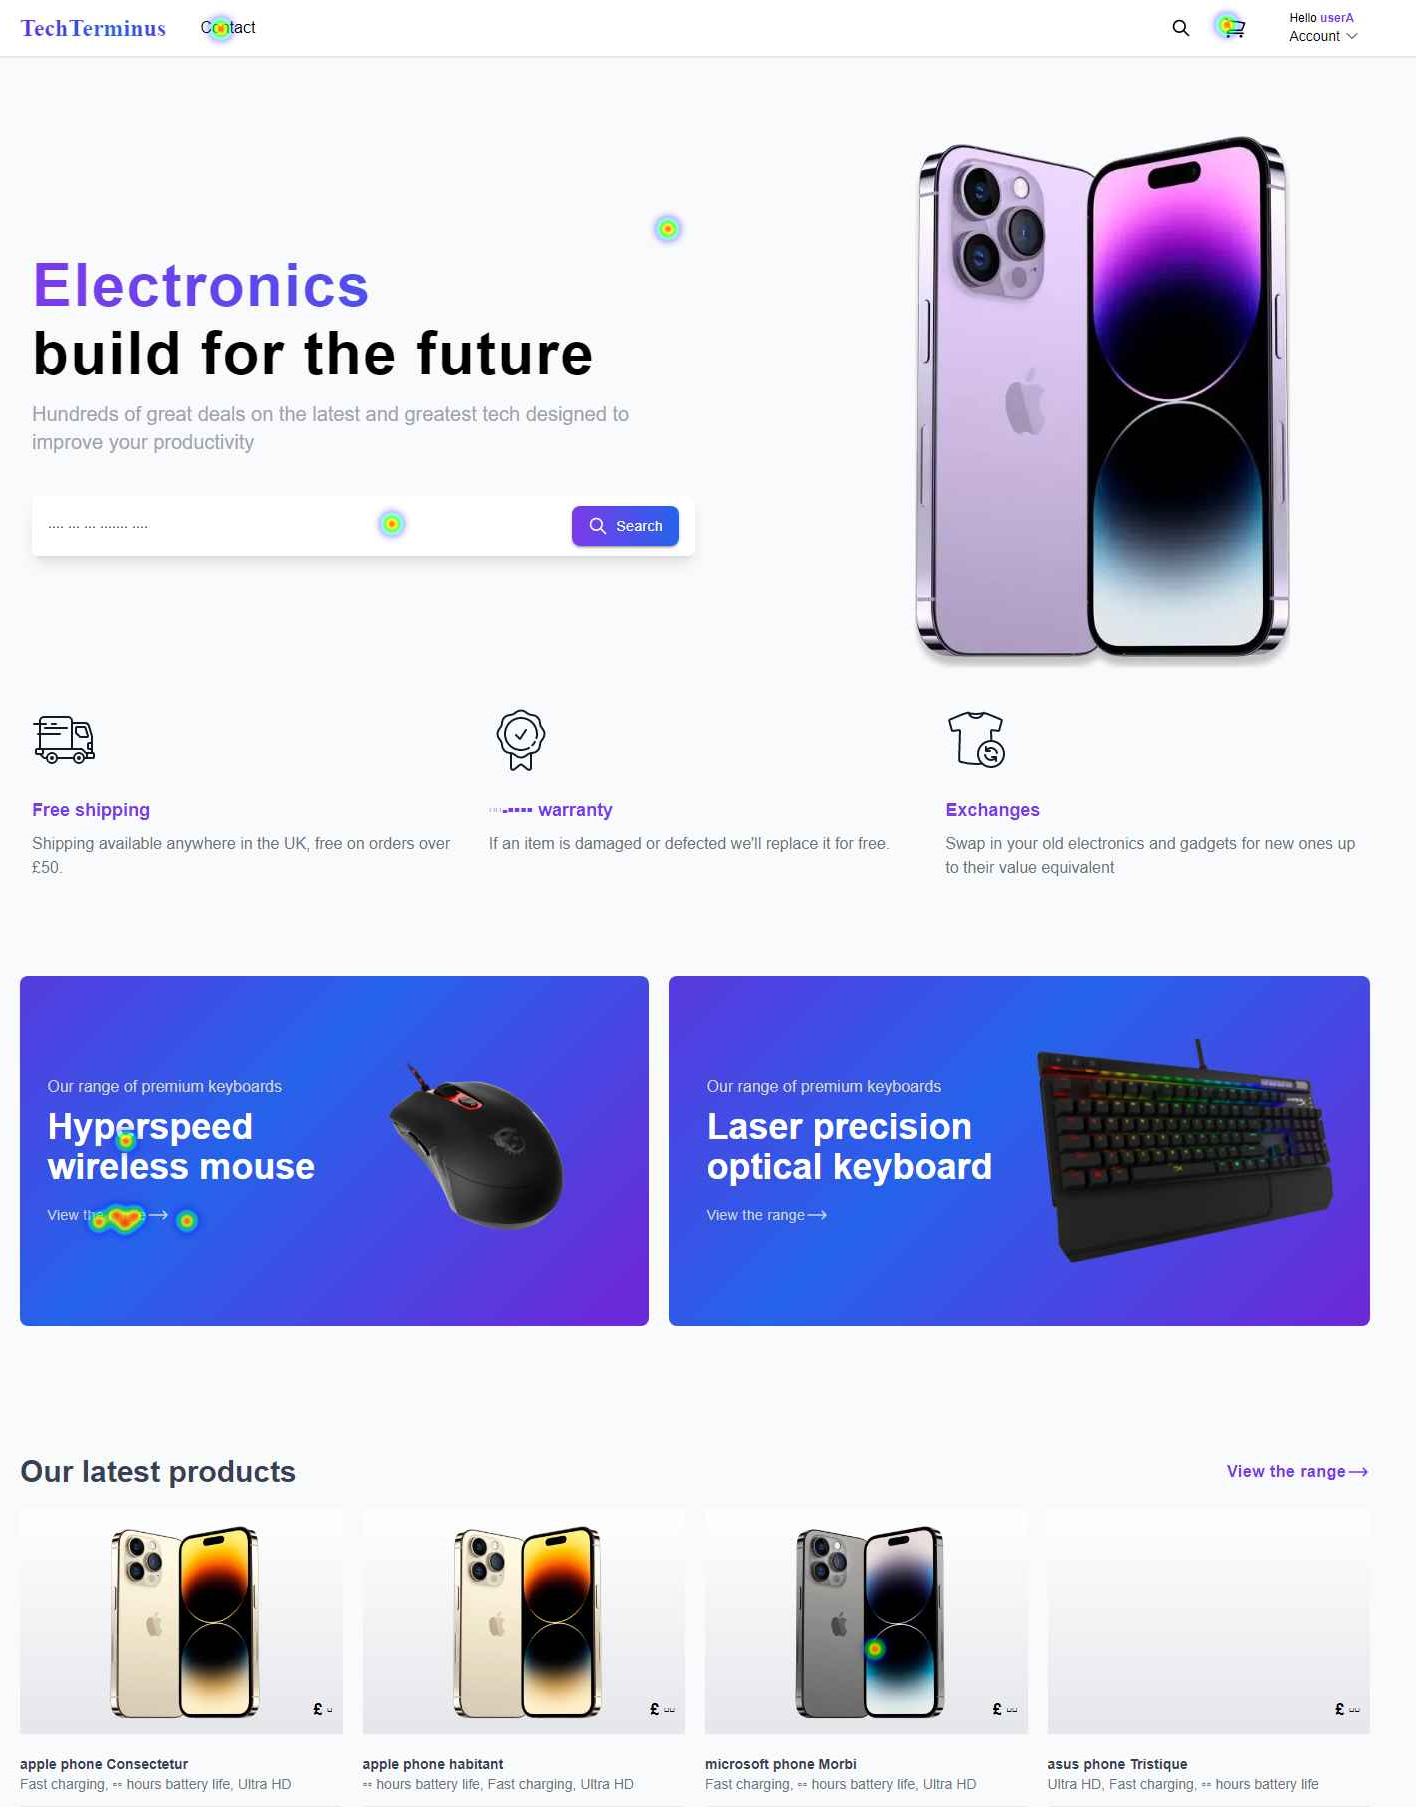
\includegraphics[width=9cm,height=9cm,keepaspectratio]{images/data/heatmap.png}
            \label{fig:heatmap}
        \end{figure}

    \section{Discussion}
        As summarised in the findings section, the hypothesis of a significant difference between the proportions of negative and positive results was proved by both artefacts when subject to a two-sample proportional test, with artefact B showing a greater difference in proportion than artefact A. However, it is important to note the limitations of the sample size and the increased impact from client related metrics. Despite these factors, the established results allow for the addressing of each research question. 
        
        \subsection{What are the most effective design elements for improving the UX of web applications?}
            Looking at the themes identified in the  findings, any back-end functionality such as error handling or performance are irrelevant to this question. While they do improve UX, they should be treated application requirements rather than areas of design refactoring that could improve UX. As a result, client-side metrics should be the main area of discussion. The heatmap data can further narrow this question as it establishes that elements on the first page load received the most clicks [\autoref{fig:heatmap}] and therefore, should have the strongest design. Papers analysed by Sudiana et al and Udo et al, in their research narrow the key elements of this first page to "colour scheme", "typography" and "ease of use" \cite{sudiana, udo}. All of these categories are supported by the results, showing that for the relevant metrics: "colour scheme", "typography and relevant information" and "accessibility" showed the greatest area of fluctuation between the two artefacts within the client-side metrics, with "ease of use" being further supported by the work of Nevarez \cite{nevarez}. 
            
            The colour scheme should match the theme of the website itself, as this is derived from the personal need for colour to match the environment. Referring to the previous example under this same research question an environmental website should use green or brown colours as this best matches its theme. The connotations of a colour should also reflect the audience and theme of the website. In this case artefact B received more negative responses because its colour scheme was "too dark" and made the site feel "unwelcoming" [appendix: \autoref{tab:study-data}]. This may have been because if perceived poorly, black can have connotations of "evil and death" rather than "sophistication and drama" \cite{lanyi}. .
            
            The typography follows a similar format. It should be a font that is both easy to read and fits the theme of the website. For example, a San Serif font would fit an online broadsheet newspaper, but it would not be very effective on a online magazine \cite{shaikh}. Artefact A used a monospace font which is often associated with technology \cite{shaikh} whereas a artefact B used a more modern font, despite both sites being e-commerce for technology products, which consequently, aside from individual preference, may have caused the increased negative results. 
            
            Ease of use is the most general and standardised of the three metrics, like the back-end metrics. Ease of use is more of a standard rather than an area that can be improved. As a result, users expect features like reaching their goal in three clicks or having a navigation bar to change pages. Developers should consider the functionality of their systems and conforming to accessibility features like ARIA and use heuristics evaluations to identify and areas of weakness and refactor them.

        \subsection{How can these design elements be understood by a non-
technical audience?}
            Now that the key elements of creating a successful UX have been discussed they can be applied to elements. For a non technical audience ease of use can be understood as the quality of usability in a site. If the usability of the site is poor users wont be able to complete their objective like buying products because the UI itself has limited functionality that cuts off certain features in the site or stops the correct features interacting. This is why this is such an important standard because even if all the other discussed metrics are outstanding it wont matter if they cannot be accessed at all. With non-technical developers often using website builders this negates the effects of poor ease of use. Pre-built components available in these tools are rigorously tested and comply with modern accessibility features, meaning that it is unlikely this group of developers will encounter any issues with ease of use, if they do they can request that the components be refactored by the developers of the web building tools they use. Regardless key elements to maintain ease of use include; having a header at the top of the page with page navigation, the logo being in the top left and links being in the top right as eye tracking suggests \cite{nevarez} and the amount of clicks needed for a user to reach their destination should be kept at a minimum, often this is referred to as the three-click rule but research claims this lacks validity \cite{porter, iglesias}.

            The Colour scheme and typography are far more subjective and less general than ease of use. This means that despite research and common themes, there is no one set of colours of fonts will appeal to all audiences. As highlighted in the previous section, both of these fields should be matched to the theme of the website itself. Colour can be used to orientate a user's perception and emotion. For example, a primarily red colour palette creates a sense of urgency \cite{lanyi}, which is often why it is used for error messages, whereas blue creates a theme of trustworthiness \cite{lanyi}, which is why its commonly used for buttons. Users can learn how to apply their colours correctly by first profiling their target demographic through their requirements as users and their likely interests and hobbies. 
            
            From this data, developers can assume a matching theme and apply a colour palette that correctly relates to the emotional response they want their website to create. In the case of artefact A, the target audience was users of technology, who are likely creative. Therefore, purple, with connotations to creativity, was chosen as the primary colour, and blue was chosen as the secondary colour. Because e-commerce websites often requires payment and processing, using blue's theme of trust increases the chance of users buying products. Website builders often have entire themes available, like artefact B but based on its higher proportion of negative results for the colour scheme metric [\autoref{fig:group-b-plots}], it is still the designer's responsibility to understand its target audience.

            Typography follows on from the colour scheme, using the established demographic along with specific accessibility requirements for its application. Any font used should be easy to read and clear enough to draw users to certain page section. This is often why large letting and bold fonts are used on the first web page to attract users to the call to action, given its importance evidenced by heatmap \autoref{fig:heatmap}. The choice of lettering is also key. For example, a website for a younger audience would use a simplistic and relaxed font style compared to a energetic themed website. Visually impaired users may require additional clarity from the font, therefore it must be clearly visible against the colours used in the site to not impact their accessibility or screen readers. Web builder themes come with built-in fonts designed to match the website. However, it still falls to the designer to optimise the font for clarity and accessibility as despite artefact B using the most optimised font for its site, it still received a slightly larger proportion of negative responses [\autoref{fig:group-b-plots}]. \\

        \subsection{Future works}
            A possible area of future research could be to investigate back-end metrics. Although this study found them difficult for participants to notice, research could be conducted to determine the best strategies to optimise back-end systems, such as error handling or performance from qualitative data to improve UX past front-end metrics. Furthermore, since colour scheme, typography and ease of use were the key metrics in this study research could solely on these metrics. For example, comparing artefacts with purposely varied colour schemes or typography could test the impact of specific themes on specific demographics. Additionally, a poorly navigated artefact could be compared to a well navigated artefact to determine which areas of ease of use are the most crucial to the accessibility and usability of participants. This same study could be re-examined with its limitations mitigated, such as using a full sample size and researching client-side metrics to discover additional or different metrics for future studies. Researchers could also focus on a study that investigates how to best communicate design elements to non-technical audiences to better answer this paper's second research question.

    \section{Conclusion}
        This paper aimed to address research questions regarding the role of UI, UX, and web design in web applications. Specifically, it investigated which design elements have the greatest impact on UX and how non-technical developers using website builders could understand them. To achieve this, an A/B test was conducted comparing two e-commerce web applications, with informed design alterations made to artefact A and artefact B made with a website builder. A qualitative analysis was then performed across several key metrics testing areas of both client-side design and server-side functionality. 
        
        The results revealed that not all metrics have the same impact. Server-side metrics were found to be more difficult for users to detect and less likely to interact with. Therefore, it is recommended that these metrics be treated as standards rather areas of design for non-technical users, ensuring that they are not neglected despite their lower impact. On the other hand, client-side metrics; "colour scheme", "typography" and "ease of use" [\autoref{tab:metrics-table}] had the greatest difference in proportions of positive and negative responses when subject to a two-sample proportional test and supported an earlier hypothesis [\autoref{tab:hypotheses}] of differing proportions between artefacts. Hence, these should be the primary focus for developers using web builder tools. Ease of use overlaps with server-side metrics in that it's more of a standard than design metric, colour scheme and typography were found to be heavily influenced by individual preference. Consequently, developers should aim to match these attributes to the theme and content of the website based on it's target audience to orientate these metrics.
        
        Although this research had a limited sample size of 42 out of 52 participants, it's data still holds some merit. However, it should be noted that participants had a greater effect size than would be standard for the full sample size. With these considerations in mind, future research should focus on the impact of server-side metrics. Research could help understand how these metrics could be utilised like the key client-side metrics in this study. Additionally, varied colour schemes and typographies should be closely examined to determine their best method of application. Finally, proper methodologies for communicating technical metrics to non-technical audiences could be utilised based on the findings of this paper and subsequent research.

    \begin{thebibliography}{9}
        % Introduction %
        \bibitem{provost}
            G. Provost and J.-M. Robert, “The Dimensions of Positive and Negative User Experiences with Interactive Products,” 2013.
        \bibitem{internet}
            Internet Live Stats, “Total number of websites - internet live stats,” Internetlivestats.com, 2018. https://www.internetlivestats.com/total-number-of-websites
        \bibitem{w3}
            “Usage Statistics and Market Share of WordPress, May 2020,” w3techs.com. https://w3techs.com/technologies/details/cm-wordpress
        \bibitem{pillai}
            A. Pillai, K. Shinohara, and G. W. Tigwell, “Website Builders Still Contribute To Inaccessible Web Design,” The 24th International ACM SIGACCESS Conference on Computers and Accessibility, Oct. 2022, doi: 10.1145/3517428.3550368.
        \bibitem{ndukwe}
            W. Ndukwe and K. Talonpoika, “Title Website Builders: A Tool In Web Design From A Graphic Design Perspective Number of Pages 53 pages + 0 appendices Degree Bachelor of Arts and Culture Degree Programme Media Specialisation Option Graphic Design Instructor(s) Keywords,” 2019. 
        \bibitem{mohd-any}
            A. A. Mohd-Any, H. Winklhofer, and C. Ennew, “Measuring Users’ Value Experience on a Travel Website (e-Value): What Value Is Cocreated by the User?,” 2015.
        \bibitem{lynch}
            P. J. Lynch and S. Horton, Web Style Guide: Foundations of User Experience Design. Yale University Press, 2016.
        \bibitem{morville}
            P. Morville, “User Experience Design,” Semantic Studios, Oct. 11, 2016.
        \bibitem{cai}
            L. Cai, X. He, Y. Dai and K. Zhu, "Research on B2B2C Ecommerce Website Design Based on User Experience," Journal of
            Physics: Conference Series, vol. 1087, no. 6, pp. 1-5, 2018.
‌
        % Literature review %
            \bibitem{udo}
                G. J. Udo and G. P. Marquis, “Factors Affecting E-Commerce Web Site Effectiveness,” Feb. 2016.
‌           \bibitem{turban}
                E. Turban and D. Gehrke, “Determinants of e‐commerce Website,” Human Systems Management, vol. 19, no. 2, pp. 111–120, 2019.
            \bibitem{sudiana}
                Sudiana, Y. U. Chandra, and L. Angela, “Key Success Factors for a Better User Experience in E-Commerce Website,” 2021 International Conference on Information Management and Technology (ICIMTech), Aug. 2021, doi: 10.1109/icimtech53080.2021.9535076.
                
            % The importance of e-commerce %
            \bibitem{slywotzky}
                Slywotzky, A.J. "The future of commerce",Harvard Business Review, January-February, 2000.
            \bibitem{ngamba}
                M. Ngamba, “E-commerce Website Design,” 2001.
            \bibitem{ullah}
                S. E. Ullah, T. Alauddin, and H. U. Zaman, “Developing an E-commerce website,” IEEE Xplore, Jan. 01, 2016. 
            \bibitem{kim}
                Kim, S., Shaw, T. and Schneider, H., "Web site design benchmarking within industry groups", 2003.
            \bibitem{merwe}
                R. van der Merwe, “A framework and methodology for evaluating e-commerce Web sites,” Dec. 2003.
            \bibitem{cuncliffe}
                Cunliffe, D, "Developing usable Web sites – a review and model", 2000.

            % Design methodologies %
            \bibitem{bryant}
                J. Bryant and M. Jones, “Responsive Web Design,” Pro HTML5 Performance, 2013.
            \bibitem{mohamed}
                A. Mohamed and R. Rimiru, “Responsive Web Design in Fluid Grid Concept Literature Survey,” 2014.
            \bibitem{harb}
                E. Harb, P. Kapellari, S. Luong, and N. Spot, “Responsive Web Design.”
            \bibitem{subnic}
                N. Subić and T. Krunić, “Online Journal of Applied Knowledge Management A Publication of the International Institute for Applied Knowledge Management Responsive web design – Are we ready for the new age?,” vol. 2, no. 1, 2014.
            \bibitem{margea}
                Margea R., Margea C., Bogdan, and Călin, “Mobile First. Current Trends and Practices in Website Design,” 2017.
            \bibitem{karolic}
                B. Karolić, “Online Journal of Applied Knowledge Management A Publication of the International Institute for Applied Knowledge Management Increasing the availability of information using modern technologies of the open Web to build user interfaces for mobile devices,” 2013.
            \bibitem{wan}
                H. A. Wan, “Opportunities to enhance a commercial site,” 1999.
‌
            % Scoping UX %
            \bibitem{law}
                E. L.-C. Law, V. Roto, M. Hassenzahl, A. P. O. S. Vermeeren, and J. Kort, “Understanding, scoping and defining user experience,” Proceedings of the 27th international conference on Human factors in computing systems - CHI 09, 2009, doi: 10.1145/1518701.1518813.
            \bibitem{schaik}
                E. L.-C. Law, P. van Schaik, and V. Roto, “Attitudes towards user experience (UX) measurement,” International Journal of Human-Computer Studies, vol. 72, no. 6, pp. 526–541, Jun. 2014, doi: 10.1016/j.ijhcs.2013.09.006.
            \bibitem{brenyon}
                D. Benyon, “A guide to HCI, UX and interaction design DESIGNING USER EXPERIENCE.”
            \bibitem{allam}
                A. Allam, A. Razak, C. Hussin, and H. Dahlan, “User Experience: Challenges and Opportunities.”
            \bibitem{vermeeren}
                A. P. O. S. Vermeeren, E. L.-C. Law, V. Roto, M. Obrist, J. Hoonhout, and K. Väänänen-Vainio-Mattila, “User Experience Evaluation Methods: Current State and Development Needs,” 2010.
            \bibitem{TAS}
                “Technology Acceptance Model - an overview | ScienceDirect Topics,” Sciencedirect.com, 2016. https://www.sciencedirect.com/topics/social-sciences/technology-acceptance-model
            \bibitem{castan}
                J. Alberto Castan˜eda, F. Mun˜oz-Leiva, and T. Luque, “Web Acceptance Model (WAM): Moderating effects of user experience§,” 2007.
            \bibitem{cao}
                M. Cao, Q. Zhang, and J. Seydel, “B2C e-commerce web site quality: an empirical examination,” 2005.

        % Research questions %
            % What are the most effective design elements for improving the UX of web applications? %
            \bibitem{ivory}
                M. Ivory and M. Hearst, “Improving Web Site Design,” 2002. Available: https://flamenco.berkeley.edu/papers/tango-ieee.pdf
                
            % How can these design elements be understood by a non-technical audience? %
            \bibitem{wijaya}
                A. Wijaya, Kefry, W. Wihalim, and A. A. Santoso Gunawan, “The Effect of UI/UX Design on User Satisfaction in Online Art Gallery,” 2021 1st International Conference on Computer Science and Artificial Intelligence (ICCSAI), Oct. 2021, doi: 10.1109/iccsai53272.2021.9609764.
            \bibitem{SUS}
                usability.gov, “System Usability Scale (SUS),” Usability.gov, 2019. https://www.usability.gov/how-to-and-tools/methods/system-usability-scale.html
            \bibitem{gunawan}
                R. Gunawan, G. Anthony, Vendly, and M. S. Anggreainy, “The Effect of Design User Interface (UI) E-Commerce on User Experience (UX),” 2021 6th International Conference on New Media Studies (CONMEDIA), Oct. 2021, doi: 10.1109/conmedia53104.2021.9617199.

        % Methodology %
            % Ethics considerations %
            \bibitem{gdpr}
                GDPR, “General Data Protection Regulation (GDPR),” General Data Protection Regulation (GDPR), 2018. https://gdpr-info.eu/

        % Findings %
        \bibitem{djamasbi}
            S. Djamasbi, “Eye Tracking and Web Experience,” AIS Transactions on Human-Computer Interaction, vol. 6, no. 2, pp. 37–54, Jun. 2014
        \bibitem{nevarez}
            C. Luna-Nevarez, “Common Practices in Destination Website Design.” Nov, 2012

        % Discussion %
        \bibitem{lanyi}
            C. SIK-LÁNYI, “Choosing effective colours for web sites,” Nov. 2011.
        \bibitem{shaikh}
            A. Shaikh, B. Chaparro, and D. Fox, “Perception of Fonts: Perceived Personality Traits and Uses,” vol. 8, 2006
        ‌\bibitem{porter}
            T. Porter and R. Miller, “Association for Information Systems AIS Electronic Library (AISeL) Investigating The Three-Click Rule: A Pilot Study.”
‌       \bibitem{iglesias}
            ‌L. Jiménez Iglesias,  C. Aguilar  Paredes,  L. Sánchez  Gómez,  M Pérez­Montoro  Gutiérrez :  “User experience  and  media.  The  three  click  rule  in  newspapers’  webs  for  smartphones”. 2018
    \end{thebibliography}

    \appendix
        Repository: \href{https://github.falmouth.ac.uk/JH248828/Comp320_A1-Comp360_A1}{JH248828/Comp320\_{A1}-Comp360\_{A1}} \\

        \section*{Appendix A: Statistics addendum}
        \addcontentsline{toc}{section}{Appendix A}
            \label{tab:study-data}
            Study data: \href{https://github.falmouth.ac.uk/JH248828/Comp320_A1-Comp360_A1/tree/documentation/data}{JH248828/Comp320\_{A1}-Comp360\_{A1}/data} \\
        
            \begin{lstlisting}[style=rListingStyle, language=R, caption={R-code used to create column graphs}, captionpos=t]
library(readr)
library(magrittr)
library(tidyr)
library(dplyr)
library(ggplot2)

# Import data from CSV file, swap file read to change graph data
data <- read_csv("group-a-data.csv")
#data <- read_csv("group-b-data.csv")

# Convert wide format to long format
data_long <- pivot_longer(data, cols = -Name, names_to = "Question", values_to = "Response")

# Count the number of positive and negative responses for each question
data_counts <- data_long %>%
  group_by(Question, Response) %>%
  summarise(Count = n()) %>%
  pivot_wider(names_from = Response, values_from = Count)

# Create a data frame with the counts of positive and negative responses for each question
df <- data.frame(
  Question = factor(data_counts$Question, levels = c(
    "What was your opinion on the colour scheme?",
    "What was your opinion on the quality of the information?",
    "How easy was the site to use?",
    "How was the site's performance?",
    "Did the sites design fit your device?",
    "Were the error systems suitable and informative, if encountered?",
    "How consistent was the site's design?",
    "Did the sites features work the way you expected?"
  )),
  Positive = ifelse(is.na(data_counts$P), 0, data_counts$P),
  Negative = ifelse(is.na(data_counts$N), 0, data_counts$N)
)

# Perform a two-sample proportional test to compare the proportions of positive and negative responses between each question
prop_test_res <- prop.test(df$Positive, df$Positive + df$Negative)

# Extract p-values
p_values <- prop_test_res$p.value

# Adjust values using Benjimini-Hochberg adjustment
adjusted_p_values <- p.adjust(p_values, method = "BH")

# Add adjusted p-values to the prop.test object
prop_test_res$p.value <- adjusted_p_values

# Plot the counts as a column chart
ggplot(df, aes(x = Question)) + 
  geom_col(aes(y = Positive, fill = "Positive"), position = position_dodge(width = 0.4), width = 0.6) + 
  geom_col(aes(y = Negative, fill = "Negative"), position = position_dodge(width = 0.4), width = 0.6) + 
  scale_fill_manual(values = c("Positive" = "#808080", "Negative" = "#000000"),
                    labels = c("Positive", "Negative")) +
  xlab("Metrics") +
  ylab("Number of responses") +
  ggtitle("UX opinion by metric") +
  scale_y_continuous(breaks = seq(0, 26, 2)) +
  theme(plot.title = element_text(hjust = 0.5, vjust = 1.5),
        legend.title = element_blank(),
        axis.text.x = element_text(angle = 45, hjust = 1, vjust = 1)) 
) \end{lstlisting}

        \section*{Appendix B: Artefacts}
        \addcontentsline{toc}{section}{Appendix B}        
            \begin{figure}[H]
                \caption{Artefact A index page \\\hspace{\textwidth} Viewable here: \href{http://www.tech-terminus.me/}{Tech Terminus}}
                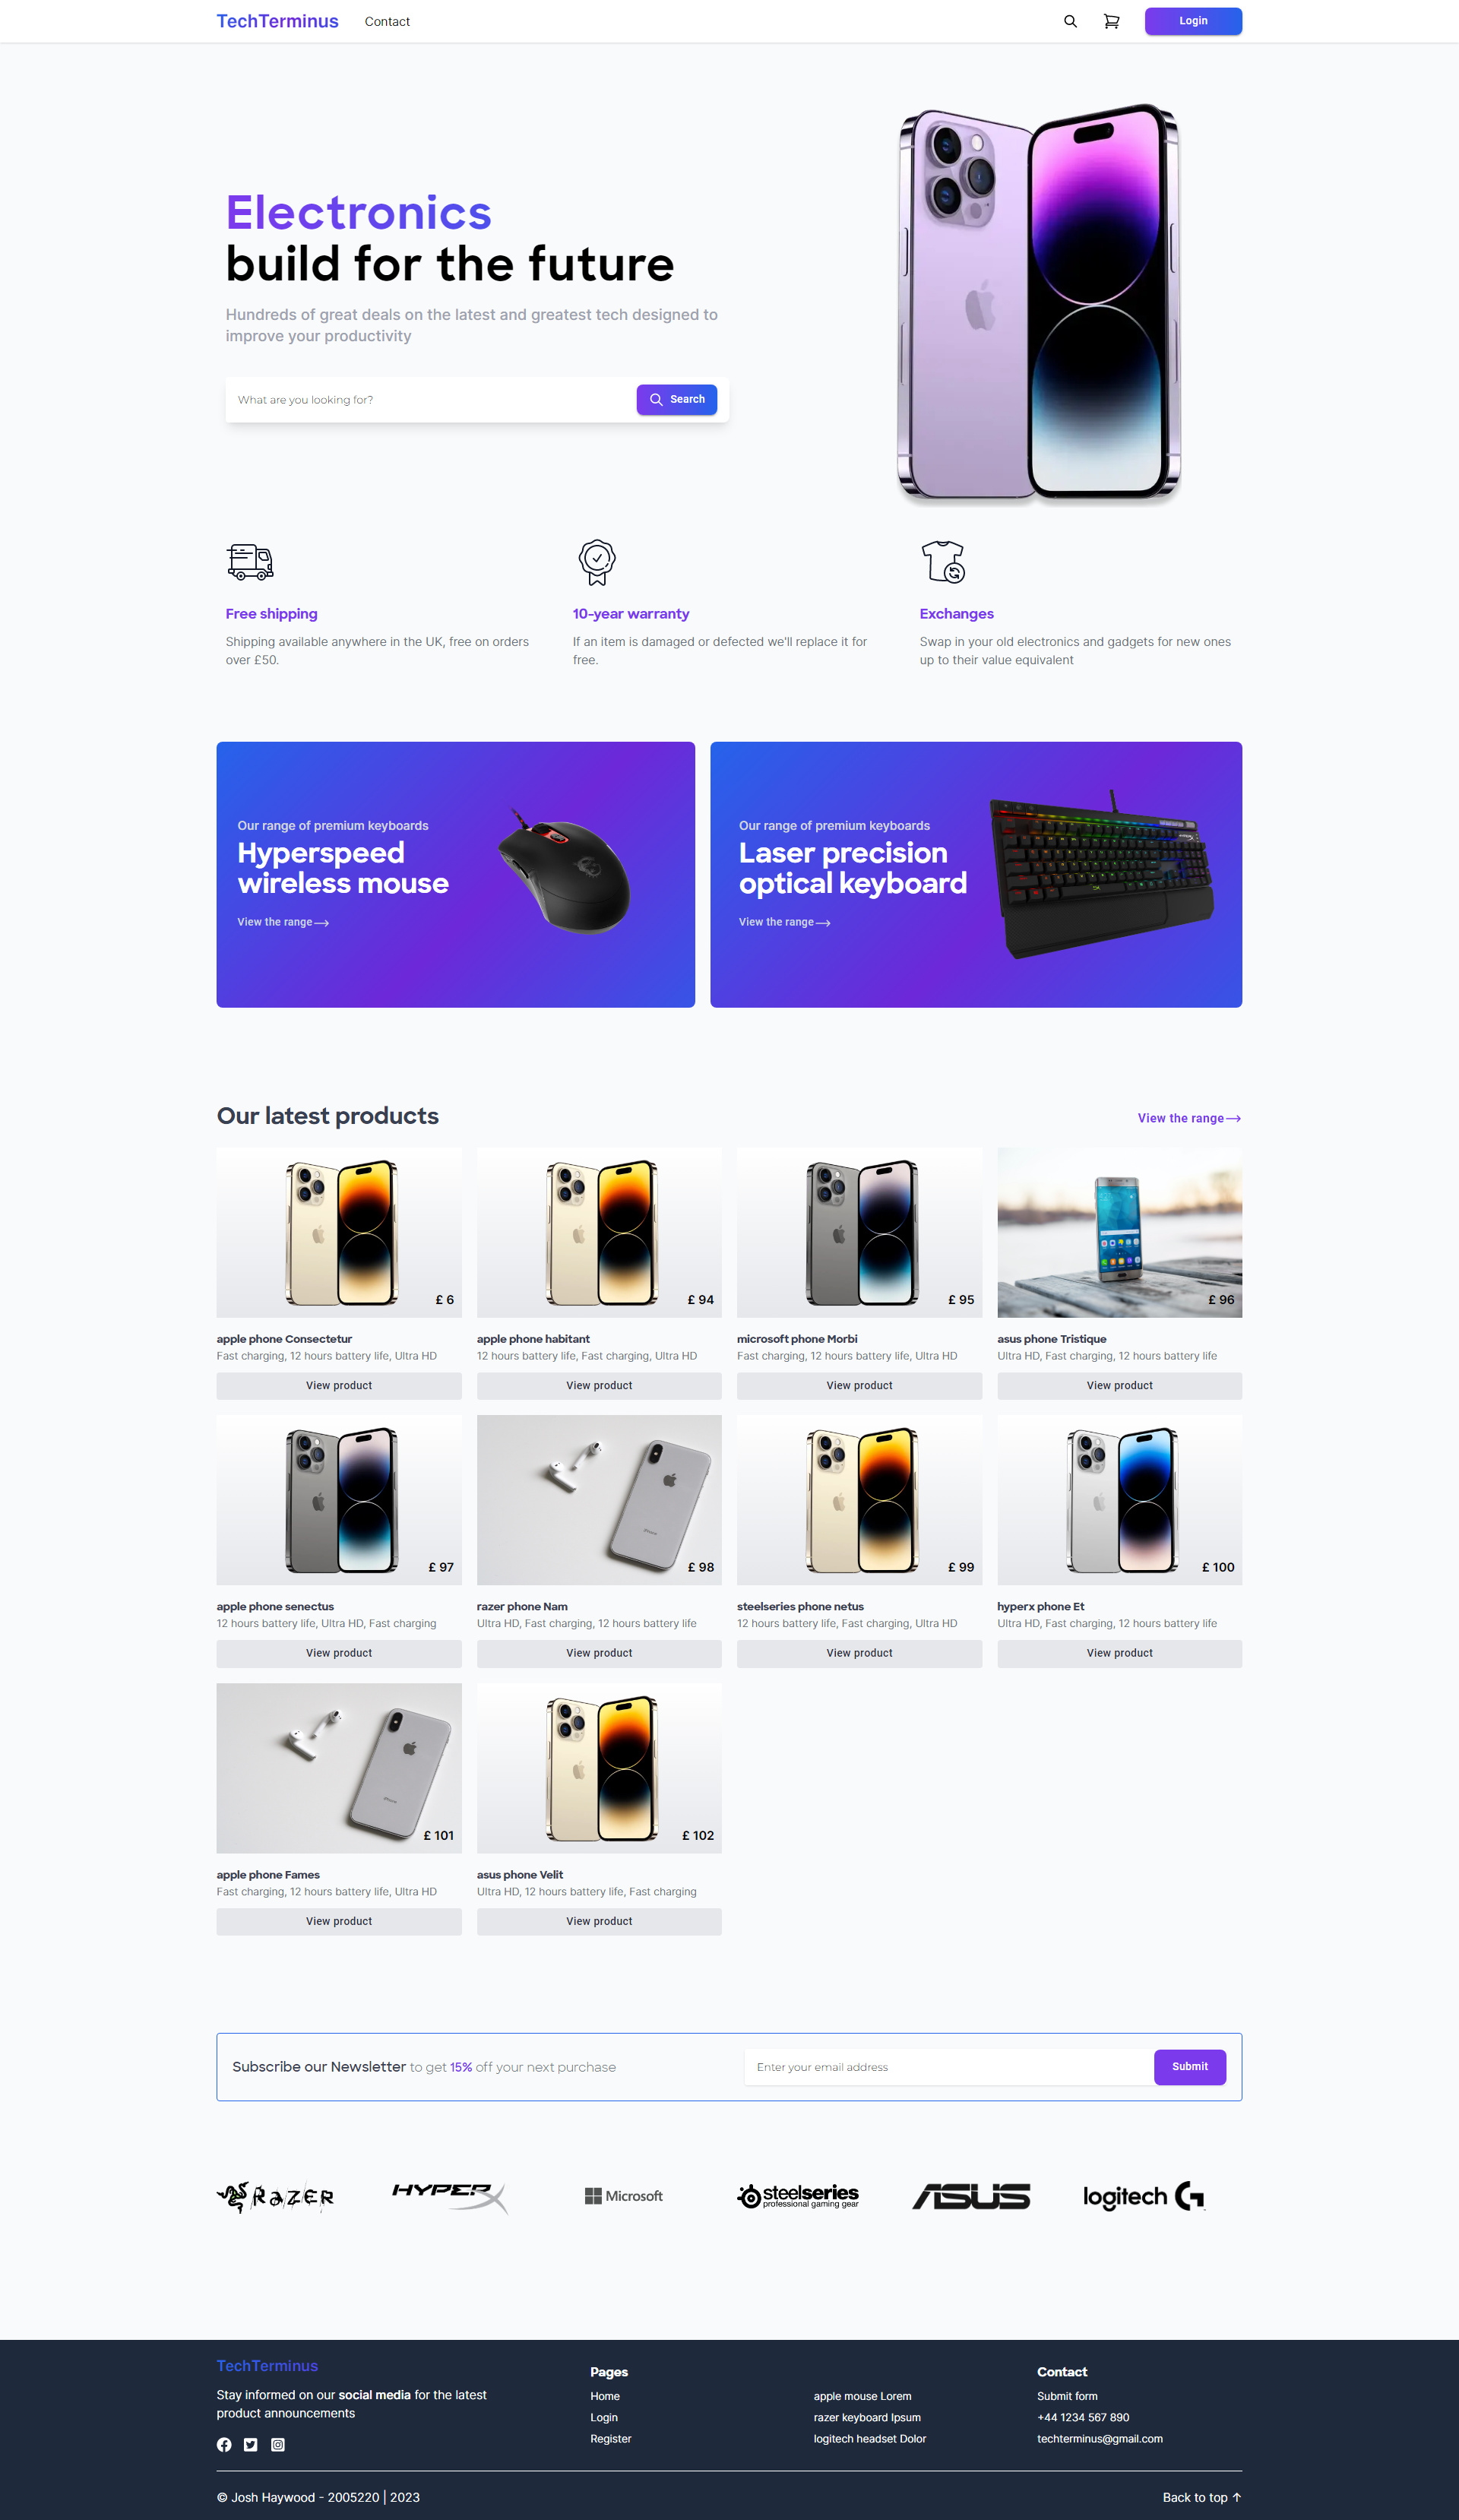
\includegraphics[width=\columnwidth]{images/artefact/artefact-a-fullpage.png}
            \end{figure}
        
            \begin{figure}[H]
                \caption{Artefact B index page \\\hspace{\textwidth} Viewable here: \href{https://beyours-theme-tech.myshopify.com/}{Shopify theme}}
                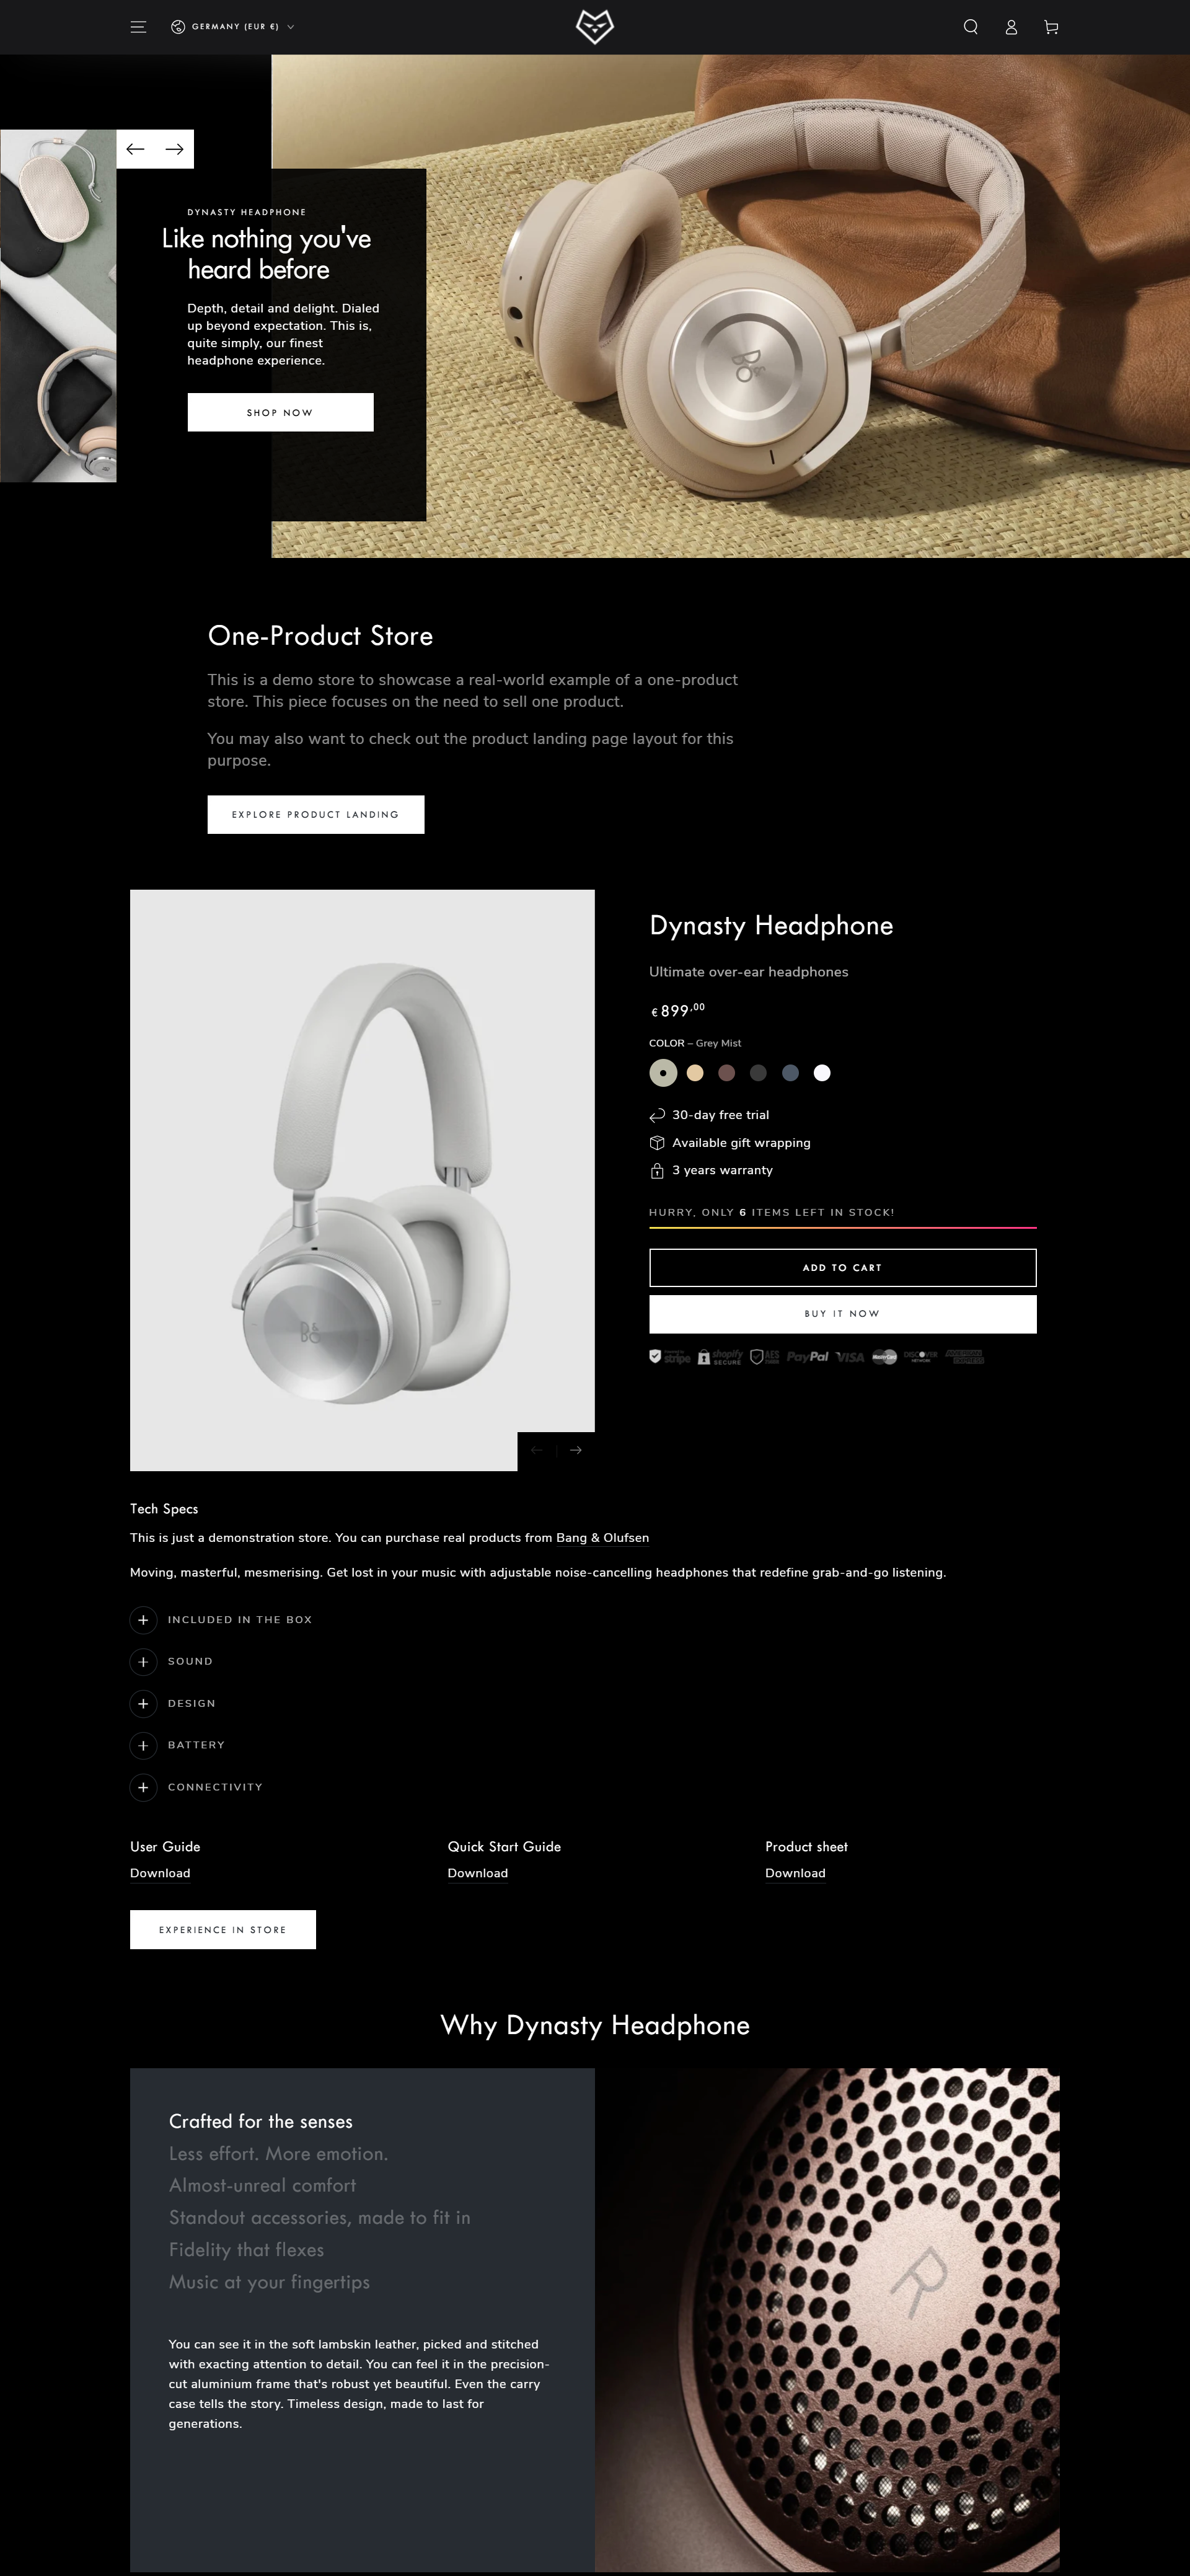
\includegraphics[width=\columnwidth]{images/artefact/artefact-b-fullpage.png}
            \end{figure}

        \section*{Appendix C: Artefact Testing Addendum}
        \addcontentsline{toc}{section}{Appendix C}
            Artefact A followed a testing plan for unit, integration, acceptance, and usability testing. These types of tests were chosen because they are the most relevant to the study and the artefact itself. Unit and integration tests are standard for testing individual features and their integration across the artefact, while acceptance and usability testing are best suited for studies relating to design. The unit and integration tests were written using React.js's testing library to test the search and cart features, checking their individual functionality, such as button clicks or submissions, as well as their integration with other features like the product listings or checkout page. The search test verifies that writing a query in the search input takes the user to the subsequent product page with the query they provided. The cart test checks several areas of functionality, such as getting items from the cart when loading the checkout page, individually updating the quantity of items, deleting individual items, and clearing all items from the cart. Each of these tests follows the same format of clicking the event button, such as the delete button, creating an Axios mock endpoint that matches the real functionality of the component, and using a mock product to test the outcome, in this case the mock product would display nulls values indicating it has been removed. 
            
            A secondary set of heuristics were written for acceptance testing, followed by refactors based on the outlined issues, including using ".env" variables to minimize errors in the HTTP request system, using a media query package for boolean variables since they do not update without reloading the page, and adding a cart clear endpoint to allow users to clear their entire cart at once, rather than each item individually [\autoref{fig:heuristic-analysis}]. Finally, the usability test was measured using Google's Lighthouse developer tools, which measured several key metrics [\autoref{fig:usability-test}]. In this case, accessibility is the metric that measures usability, taking into account accessibility features such as image alt text, ARIA labeling, and screen reader compatibility.

            \begin{lstlisting}[style=jsListingStyle, caption={Search functionality test}, captionpos=t]
import { render, screen, fireEvent } from "@testing-library/react";
import { BrowserRouter as Router } from "react-router-dom";

import SearchBar from "../search-bar";

test("searches for query when user inputs and submits search term", () => {
  const setSearchBar = jest.fn();
  const query = "phone"; // User input
  render(
    <Router>
      <SearchBar
        variant="hero"
        setSearchBar={setSearchBar}
        setOverlay={jest.fn()}
      />
    </Router>
  );

  const input = screen.getByPlaceholderText("What are you looking for?");
  fireEvent.change(input, { target: { value: query } });
  fireEvent.keyDown(input, { key: "Enter", code: 13, charCode: 13 }); // Simulate user pressing enter

  expect(setSearchBar).toHaveBeenCalledWith(false);
  expect(window.location.pathname).toBe(`/results/${query}`); // Expect to navigate to results page with query as ID
});
) \end{lstlisting}

            \begin{lstlisting}[style=jsListingStyle, caption={Cart functionality tests}, captionpos=t, mathescape=true]
import { render, screen, fireEvent } from "@testing-library/react";
import "@testing-library/jest-dom/extend-expect";
import { BrowserRouter as Router } from "react-router-dom";
import axios from "axios";

import Summary from "../checkout/Summary";

jest.mock("axios");

describe("Summary component", () => {
  beforeEach(() => {
    jest.clearAllMocks();
  });

  // Getting products from cart and displaying them
  it("should fetch products from cart and display them", async () => {
    const mockData = [
      {
        product_name: "Product 1",
        price: 10,
        quantity: 1,
        image: "https://example.com/product1.jpg",
      },
      {
        product_name: "Product 2",
        price: 20,
        quantity: 2,
        image: "https://example.com/product2.jpg",
      },
    ];

    axios.get.mockResolvedValueOnce({ data: mockData });

    render(
      <Router>
        <Summary />
      </Router>
    );

    // Wait for products to load
    await screen.findByText("Product 1");

    // Check if products are displayed correctly
    expect(screen.getByText("Product 1")).toBeInTheDocument();
    expect(screen.getByText("$\mbox{\pounds}$ 10")).toBeInTheDocument();
    expect(screen.getByText("Product 2")).toBeInTheDocument();
    expect(screen.getByText("$\mbox{\pounds}$ 20")).toBeInTheDocument();

    //Check if clear cart button clears cart
    //Click the clear cart button
    const clearCartButton = screen.getByRole("button", { name: /Clear cart/i });
    clearCartButton.click();

    // Wait for products to be removed
    await screen.findByText(/Your cart is currently empty/i);

    // Check if the cart is empty
    expect(screen.queryByText("Product 1")).toBeNull();
    expect(screen.queryByText("$\mbox{\pounds}$ 10")).toBeNull();
    expect(screen.queryByText("Product 2")).toBeNull();
    expect(screen.queryByText("$\mbox{\pounds}$ 20")).toBeNull();

    // Click the return button
    const returnButton = screen.getByRole("button", { name: /Return/i });
    returnButton.click();

    // Check if the user is redirected to the homepage
    expect(window.location.pathname).toBe("/");
  });

  // Update products from cart
  it("should update the quantity of a product in the cart", async () => {
    const mockData = [
      {
        product_name: "Product 1",
        price: 10,
        quantity: 1,
        image: "https://example.com/product1.jpg",
      },
    ];

    axios.get.mockResolvedValueOnce({ data: mockData });

    render(
      <Router>
        <Summary />
      </Router>
    );

    // Wait for product to load
    await screen.findByText("Product 1");

    // Click the dropdown and select a new quantity
    const quantityDropdown = screen.getByRole("combobox");
    fireEvent.change(quantityDropdown, { target: { value: "2" } });

    // Wait for quantity to update
    await screen.findByText("2");

    // Check if quantity is displayed correctly
    expect(screen.getByText("2")).toBeInTheDocument();
    expect(screen.getByText("$\mbox{\pounds}$ 20")).toBeInTheDocument();

    // Click the dropdown and select a new quantity
    fireEvent.change(quantityDropdown, { target: { value: "1" } });

    // Wait for quantity to update
    await screen.findByText("1");

    // Check if quantity is displayed correctly
    expect(screen.getByText("1")).toBeInTheDocument();
    expect(screen.getByText("$\mbox{\pounds}$ 10")).toBeInTheDocument();
  });

  // Delete products from cart
  it("should delete a product from the cart", async () => {
    const mockData = [    {      product_name: "Product 1",      price: 10,      quantity: 1,      image: "https://example.com/product1.jpg",    },    {      product_name: "Product 2",      price: 20,      quantity: 2,      image: "https://example.com/product2.jpg",    },  ];
  
    axios.get.mockResolvedValueOnce({ data: mockData });
  
    render(
      <Router>
        <Summary />
      </Router>
    );
  
    // Wait for products to load
    await screen.findByText("Product 1");
  
    // Check if products are displayed correctly
    expect(screen.getByText("Product 1")).toBeInTheDocument();
    expect(screen.getByText("$\mbox{\pounds}$ 10")).toBeInTheDocument();
    expect(screen.getByText("Product 2")).toBeInTheDocument();
    expect(screen.getByText("$\mbox{\pounds}$ 40")).toBeInTheDocument();
  
    // Find the bin SVG for the first product and click it
    const binIcon = screen.getAllByRole("img", { name: "Delete" })[0];
    binIcon.click();
  
    // Wait for product to be removed
    await screen.findByText("Product 2");
  
    // Check if the correct product was removed
    expect(screen.queryByText("Product 1")).toBeNull();
    expect(screen.queryByText("$\mbox{\pounds}$ 10")).toBeNull();
    expect(screen.getByText("Product 2")).toBeInTheDocument();
    expect(screen.getByText("$\mbox{\pounds}$ 40")).toBeInTheDocument();
  });
});
) \end{lstlisting}   

            \begin{figure}[H]
                \caption{Heuristic analysis conducted 09/03/2023 \\\hspace{\textwidth} Reference: \href{https://github.falmouth.ac.uk/JH248828/Comp320_A1-Comp360_A1/tree/documentation/hueristics}{JH248828/Comp320\_A1/documentation}}
                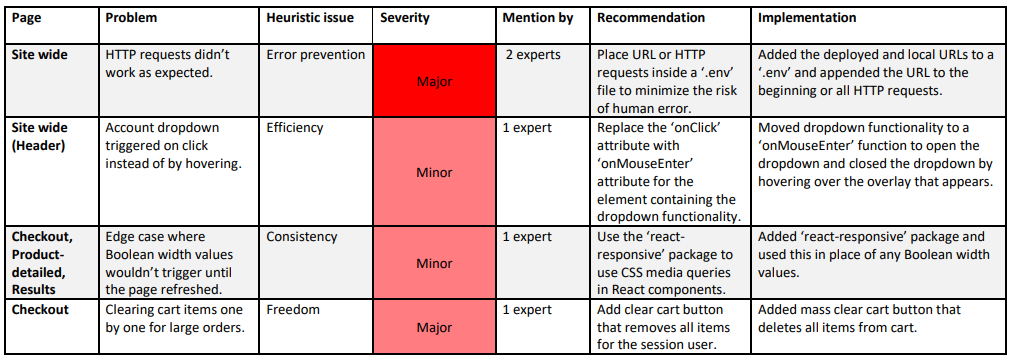
\includegraphics[width=\columnwidth]{images/testing/heuristic-analysis-block-2.png}
                \label{fig:heuristic-analysis}
            \end{figure}
        
            \begin{figure}[h]
                \caption{Lighthouse metrics \\\hspace{\textwidth} Reference: \href{https://github.falmouth.ac.uk/JH248828/Comp320_A1-Comp360_A1/tree/documentation}{JH248828/Comp320\_A1/documentation}}
                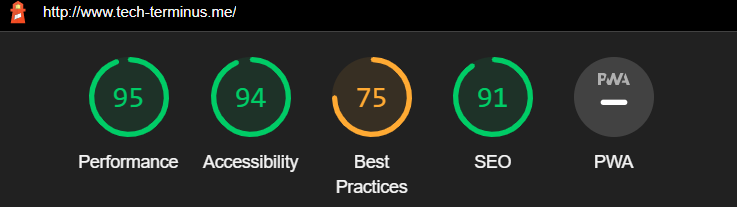
\includegraphics[width=\columnwidth]{images/testing/usability-test.png}
                \label{fig:usability-test}
            \end{figure}

        \section*{Appendix D: Critical Addendum}
        \addcontentsline{toc}{section}{Appendix D}
            Overall, the dissertation and study had merits that contributed to the area of study, and the results gathered encourage new developments. The benefits and limitations of website builders is an increasingly prevalent issue in web design, making this area of research important to developers and businesses alike. The literature review helped to encourage new areas of discussion by examining previous research such as the difficulties of scoping UX or e-commerce sites in business. The ethics and data collection plan were successful in ensuring that data was secure, and that it could be analyzed with statistical tests and presented clearly with graphs in the results and findings sections. The research questions used were relevant to the area of study, and the answers given in the discussion section could benefit future research. However, the study was not free of limitations. The sample size was insufficient, meaning the individual answers had a greater effect size than normal, rendering the data inconclusive. In hindsight, the methodology of an A/B test and qualitative questionnaire was not as effective as other methodologies, such as surveying many design papers, as other researchers had done previously \cite{sudiana, udo}.

            \subsection{Complexity of Literature review}
                The literature review presented the greatest cognitive challenge in my dissertation due to its requirements and complexity. In my opinion, the subsection on "design methodologies" could have been substituted with a more relevant subsection, such as the key principles or the significance of UI and UX in software development. These sections would have provided readers with greater insights into UI and UX for those lacking any prior knowledge and would have offered an understanding of the critical role UI and UX play in modern applications, to the extent where entire disciplines have been created around UI and UX such as web design, that focuses on efficient design to maximize UX.
            
                The irrelevance of the "design methodologies" section was likely caused by my own lack of understanding of scientific writing and literature reviews, as it was my first instance of both. With a greater knowledge of scientific literature and its structure, I can avoid re-occurrences in the future. Given that my projected career path is a web developer it is important to ensure the relevance of any work, even outside of academia, such as application documentation or presenting applications. 

                In any future academic or non-academic writing, I will allocate an additional week or fortnight to background research and ensure that the research is relevant to the literature. I will measure this by seeking feedback from peers or staff. By doing so, I will have more relevant information available for the document I am writing, enabling me to select and discard information based on its relevance rather than using loosely relevant information due to time constraints, benefiting any future documenting I may write.

            \subsection{Artefact A's design constraints}
                During the creation of artefact A, a procedural challenge arose due to the distinguishing features required for this study. The artefact needed informed design alterations based on survey papers \cite{udo, sudiana} from the literature review. With the aim of the alterations being to generate results for the study's metrics [\autoref{tab:metrics-table}]. This approach provided both direction and constraints during development, similar to the requirements of a user in industry, where the client's needs for the application define the limits of development.
    
                I was successful in implementing necessary alterations such as adjusting the colour palette, index page structure, and handling images as PNGs or with backgrounds, although this limited my creative freedom and approach during development. Additionally, I effectively followed the outlined test plan and made no deviations, however, it should have included more coverage of the core features like filtering results, but this was limited by scope.
                
                The design alterations imposed by the study restricted the development of the artefact, but this could have been avoided by assessing the limitations to development before deciding on the design options. In industry, when having requirements set out by a client they can be offset by conversing with them to alter any limitations.
    
                For future applications, I will ensure that I fully understand the application requirements. If these requirements negatively impact the development or quality of the artefact, I will access the constraints that I have set out and make changes where necessary. If developing for a client, I will converse with them and explain how the outlined requirements may impact the overall quality of the product and if individual I will access my own approach to the applications requirements. This target will benefit the quality of my applications, help build rapport with clients, and maintain my creative freedom during development. To measure the effectiveness of this target, I will assess the quality of the artefact through developer tools such as Google Lighthouse or user feedback. To ensure that it's quality has not been effected as a result of the requirements.

            \subsection{Ethical requirements and considerations}
                The ethical considerations, requirements and plan have been the greatest affective challenge during this research. The study's ethical considerations required significant preparation and thought to ensure it met all guidelines, such as GDPR. Data collected during the study was anonymized and stored securely to not breach any guidelines and there were various documents such as risk assessments, brief, debriefs and consent forms required for approval. This challenge was chosen because the software industry has many governed rules and regulations, including GDPR, which requires passwords to be encrypted and databases to be secure. Therefore, ethical considerations are prevalent throughout software applications. To follow ethical guidelines my study anonymized participant names and ensured consent forms were signed prior to taking part in the study meaning all user data correctly aligned with regulations. 
                
                The reason why this became a challenge despite the execution is that many of the aspects of ethical consideration and approval were not apparent to me when first deciding a methodology, impacting the speed of gaining approval. Therefore, in future application development, any ethics or regulations will be well considered across all aspects to ensure the applications meets their demands. This can be achieved by having correct error systems, encryption and secure data storage. The effectiveness of the ethical consideration can be measured by using test participants and checking that their data isn't accessible during any part of their experience, ensuring my applications comply with protection acts.

            \subsection{Time management}
                The greatest dispositional challenge I faced during this dissertation was time management. With so many areas to cover, from the background research and literature review to the study and research gathering, it was crucial to manage my time effectively and complete each section systematically given there were so many. This was an area I struggled with, resulting in some sections, like the literature review and methodology, receiving more time for drafting than other sections like the discussion or findings. This not only affected the overall quality of work but meant that some sections were noticeably stronger than others. 
                
                I choose to focus on time management as a challenge because is a transferable skill that is valued in industry. These same skills will need to be applied when developing and documenting any future software. My poor time management affected the study portion of the dissertation significantly. I spent too time collecting participants, which left me with less time to analyse and discuss my findings, resulting in less time to draft those sections. 
    
                To address this challenge in future work, I plan to spend more time correctly assessing the key areas of the task and breaking it down into manageable sections. Each sections will be assigned a specific amount of time based on its estimated time to complete, which will help me to ensure that no areas overlooked, and unnecessary sections are not given too much attention. I will measure the success of this approach by evaluating the overall quality of work produced and assessing my own time management during the task.

            \subsection{Task prioritization}
                Interpersonally, I found managing the dissertation and ongoing projects to be difficult. The dissertation and its proposal ran alongside the work of other modules, such as my group web application. This meant I had balance my priorities between these modules, resulting in infrequent sprints for the group project and entire weeks dedicated solely to the dissertation. While these breaks were discussed and approved as a team, they impacted the overall quality of work in other modules. In hindsight, the dissertation and other modules were balanced well throughout the study block, dedicating certain days to the dissertation while dedicating others to the group project, ensuring consistency across both. However some weeks, towards the deadline, had to be dedicated solely to the dissertation due to its closer deadline. Prioritization is common in industry,  as its very likely that multiple projects will be handled simultaneously and task delegation will have to be managed across them.
    
                To maintain the approach used during this dissertation, I will ensure that future work is assessed based on the estimated time to complete and the deadline allowed for it. Based on this assessment, work can be assigned to whichever task is more pressing while still ensuring that some work goes to the less prevalent tasks to maintain consistency. This can be measured by assessing my own performance through logging systems like GitHub's commit history to ensure that commits aren't too infrequent and having my performance evaluated by others.

            \subsection{Prioritization of artefact features}
                Similarly to my interpersonal challenge, my practice challenge was managing priorities, specifically related to the artefact. Given the design constraints I mentioned earlier, I wanted to ensure that I delivered a feature rich application to give my participants lots of tools to complete their task efficiently while staying within the design constraints. This led to the inclusion of features such as search filters and product pagination systems and updating and deleting items from the cart. Given additional scope I would have added additional pages or worked to improve the existing features, but given the complexity of the dissertation I was not able to do this. Consequently, participant feedback included requests for more quality of life features such as a mass-clear cart button or the 
                use of real product names instead of placeholders. As mentioned in the interpersonal challenge, prioritization is a key skill in industry, and this applies not only to documentation but also to software development. Developers are often faced with the challenge of balancing user requirements against their own feature ideas and decisions that they believe would improve the application.
    
                To combat this challenge in future projects, the best approach is either to allocate more time to the artefact's development or to increase the project's scope. However, since extra time is not always feasible, negotiations with clients or project managers may be necessary. The  effectiveness of the solution can be evaluated by my own satisfaction with the available featured or, preferably, through heuristic evaluations and user feedback. This feedback can be used to understand user requirements and incorporate additional or refactor current features. \\

            In conclusion, a dissertation is a highly complex and time-consuming undertaking that requires careful consideration of its many aspects and avenues, particularly when creating an artefact to accompany it. The conductor must understand each of the complex sections, manage them appropriately along side other tasks, and create an artefact that incorporates the desired study requirements without compromising UX or breaching the study's constraints. In hindsight, the dissertation was executed well despite complexity and addressed the research questions effectively. However, I have the identified several areas for improvement in future work, whether scientific literature or industry related: Fully understanding the requirements of the task before undertaking it, including both the writing sections and any constraints set by the corresponding software, legislation or regulations; effectively managing time throughout the process and prioritizing more complex tasks appropriately; and ensuring that no ongoing work is negatively impacted by the delegation of time towards the present task.
\end{document}